\documentclass[12pt,british,twoside,notitlepage,usenames,dvipsnames,hypens,final]{report}
%% Page setup
\usepackage[a4paper, twoside]{geometry}
\geometry{verbose,tmargin=3cm,bmargin=3cm,lmargin=2.5cm,rmargin=2.5cm,headheight=3cm,headsep=0.5cm,footskip=1.5cm}
\usepackage[unicode=true,
 bookmarks=true,bookmarksnumbered=true,bookmarksopen=true,bookmarksopenlevel=1,
 breaklinks=false,pdfborder={0 0 0},backref=false,colorlinks=false]
 {hyperref}
\hypersetup{pdftitle={Video Steganography using Motion Vectors -- CST Part II dissertation}, pdfauthor={E Liberis}}

\addtolength{\oddsidemargin}{6mm}
\addtolength{\evensidemargin}{-8mm}

\raggedbottom
\sloppy
\clubpenalty1000%
\widowpenalty1000%

%% Font and text flow setup
\usepackage{amsthm}
\usepackage{amsmath}
\usepackage{amssymb}
\usepackage{array}
\usepackage{afterpage}

\usepackage{polyglossia}
\setdefaultlanguage[variant=british]{english}

\usepackage{sectsty}
\allsectionsfont{\sffamily}

\usepackage{fontspec}
\setmainfont[Mapping=tex-text, Ligatures=TeX]{TeX Gyre Pagella}
\setsansfont[Mapping=tex-text, LetterSpace=1]{Gillius ADF}
\setmonofont[Mapping=tex-text]{Latin Modern Mono}

\usepackage{setspace}
\setstretch{1.1}

\setlength{\parskip}{0.5\baselineskip}
\setlength{\parindent}{0pt}

\usepackage{pifont}
\usepackage{graphicx}
\usepackage{wrapfig}
\usepackage{pstricks-add}
\usepackage{subcaption}
\usepackage[section]{algorithm}
\usepackage{algpseudocode}

%% List setup
\renewcommand\thesubsection{\arabic{subsection}.}
\usepackage{enumitem}
\setlist{nolistsep}
\setitemize{itemsep=2pt,topsep=0pt,parsep=5pt,partopsep=0pt}

%% Misc appearance things
\usepackage{pdfpages}
\newtheorem{definition}{Definition}
\numberwithin{equation}{section}
\numberwithin{figure}{section}
\usepackage{multicol}
\usepackage{alltt}
\let\oldalltt\alltt
\renewenvironment{alltt}{\vspace{-0.6\baselineskip}\begin{oldalltt}}{\end{oldalltt}\vspace{-0.1\baselineskip}}

\usepackage{titlesec}
\titlespacing\section{0pt}{4pt plus 0.5pt minus 0pt}{0pt plus 0.5pt minus 0.5pt}
\titlespacing\subsection{0pt}{5pt plus 4pt minus 2pt}{0.5pt plus 0.5pt minus 0.5pt}
\titlespacing\subsubsection{0pt}{5pt plus 4pt minus 2pt}{0.5pt plus 0.5pt minus 0.5pt}

\newcommand*\circled[1]{\tikz[baseline=(char.base)]{
            \node[shape=circle,draw,inner sep=2pt] (char) {#1};}}
\titleformat{\chapter}[hang]{\Huge\sf\bfseries}{\scalebox{2}{\circled{\thechapter}}}{1cm}{\Huge\bfseries}

\usepackage{epigraph}
\setlength{\epigraphrule}{0pt}

\usepackage{titletoc}
\titlecontents{chapter}% <section-type>
  [0pt]% <left>
  {\addvspace{1em}}% <above-code>
  {\sf\bfseries\chaptername\ \thecontentslabel:\quad}% <numbered-entry-format>
  {\sf\bfseries\thecontentslabel}% <numberless-entry-format>
  {\bfseries\hfill\contentspage}% <filler-page-format>
  []

\usepackage[labelfont=bf,width=0.9\textwidth]{caption}
\usepackage{emptypage}

%% Some useful macros
\newcommand{\arr}{\textrightarrow\ }
\newcommand{\textsb}[1]{\textsf{\textbf{#1}}}
\newcommand{\textsbc}[1]{\sffamily \textsc{\textbf{#1}}}
\usepackage{lipsum}
\usepackage{tikz}

%%%%%%%%%%%%%%%%%%%%%%%%%%%%%%%%%%%%%%%%%%%%%%%%%%%%%%%%
\begin{document}

%% Title Page
\pagestyle{empty}

\hfill{\LARGE Edgaras Liberis}

\vspace*{60mm}
\begin{center}
\Huge
{\bf Video Steganography \\ using Motion Vectors} \\
\vspace*{10mm}
{ \sc \LARGE
Computer Science Tripos, Part II \\
Homerton College \\
}
\vspace*{10mm}
\the\year 
\end{center}

\cleardoublepage

%% Proforma
\pagenumbering{arabic}
\setcounter{page}{3}
\pagestyle{plain}

{\section*{\Huge Proforma}}

{\large
\begin{tabular}{ll}
Name:               & \bf Edgaras Liberis                          \\
College:            & \bf Homerton College                         \\
Project Title:      & \bf Video Steganography using Motion Vectors \\
Examination:        & \bf Computer Science Tripos Part II, 2016    \\
Word Count:         & \bf 9099\footnotemark[1]                     \\
Project Originator: & Edgaras Liberis                              \\
Supervisor:         & Daniel Thomas                                \\ 
\end{tabular}
}
\footnotetext[1]{This word count was computed
by {\tt detex -n el398\_dissertation.tex | tr -cd '0-9A-Za-z $\tt\backslash$n' | wc -w}
}
\stepcounter{footnote}
\vspace{0.5cm}

\section*{Original Aims of the Project}

The aim of this project is to implement and evaluate various approaches to motion vector steganography. Both motion vector-specific approaches and the application of other steganographic methods to motion vectors are considered. To achieve this, an end-user tool should be developed to offer several steganographic methods. The algorithms will be evaluated based on criteria such as embedding capacity, speed, and detectability. A suite of steganalysis tools will be created.  

\section*{Work Completed}

Applications for embedding and extracting data from motion vectors were developed, providing several popular LSB steganography algorithms. Several steganalysis methods were implemented to extract and analyse motion vectors, offering classic and motion vector-specific attacks against embedding schemes. The algorithms were compared against each other evaluating detectability, capacity and other aspects, and a human study was conducted to evaluate detectability.

\section*{Special Difficulties}

None.

\cleardoublepage

%% Declaration of Originality
\section*{Declaration of Originality}
I, Edgaras Liberis of Homerton College, being a candidate for Part II of the Computer Science Tripos, hereby declare that this dissertation and the work described in it are my own work, unaided except as may be specified below, and that the dissertation does not contain material that has already been used to any substantial extent for a comparable purpose.

\bigskip
\leftline{\bf Signed }

\medskip
\leftline{\bf Date}

\cleardoublepage
\tableofcontents
%% Chapters
\renewcommand{\thesection}{\arabic{chapter}.\arabic{section}}
\renewcommand{\thesubsection}{\arabic{chapter}.\arabic{section}.\arabic{subsection}}
\setcounter{chapter}{0}

% Introduction
\cleardoublepage
\chapter{Introduction}
\pagestyle{headings}

\section{Motivation}
\label{motivation}

\emph{Steganography} is the art of concealing information within ostensibly innocent carrier data~\cite[p.~3]{fridrich}, usually with the intention of creating a covert channel. Its applications include bypassing government censorship, avoiding law enforcement or military intelligence, and other situations in which detection of the communication may be harmful to the communicating parties (such as by revealing their location~\cite{infohiding-survey}). 

Steganography research has explored the use of mainstream digital media formats as the carrier data for hidden messages. These formats often exhibit a significant degree of redundancy which provides opportunities for payload concealment~\cite[p.~2]{fridrich}. Since multimedia formats have become so widespread online, their use is now unremarkable and unlikely to raise suspicion.

By hiding data in regions of a file that are highly tolerant to small modifications or noise, the likelihood of detection can be significantly reduced. This concept led to the development of the common \emph{least-significant-bit (LSB) embedding}~\cite{bateman}\label{lsb-steg} technique, which uses the least significant bit of each data element (such as the colour channels in an image pixel) to store the payload.

This project considers the use of video files as the carrier data. The MPEG\footnote{Moving Picture Experts Group.} video compression format exploits the temporal redundancy of video frames by encoding the difference between frames as a set of motion vectors (to represent translation) and prediction errors (to represent image changes in addition to the translation). Due to the lossiness of this encoding, motion vectors are fairly noise-tolerant, so provide opportunities for hiding a payload.

To evaluate a steganographic algorithm, we need to determine if its use is detectable by an adversary. The study of methods of detecting steganographic manipulations is called \emph{steganalysis}. Steganalysts use various domain-specific statistical attacks, such as plotting histograms, looking for correlations (or lack thereof) in the data, \emph{etc.} to detect the hidden message.

This project explores hiding data in the motion vectors of MPEG videos by applying LSB embedding to the $x$ or $y$ components of the vector. A tool was developed to offer several high-capacity data embedding algorithms and encryption with a user-provided password. These algorithms were evaluated based on embedding capacity, speed, and detectability (using statistical steganalytic methods implemented in Matlab).

\section{Existing work}
Traditionally, image steganography has received more research attention than video steganography, so early attempts tried to directly apply existing image (JPEG) steganography techniques~\cite{bateman, jpegdctcoding} to video frames.

Bateman reviews the evolution of LSB-based embedding algorithms~\cite{bateman}. Simple strategies such as changing the intensity of every pixel are destroyed by the lossiness of image compression when an image is recompressed. One approach for solving this was to modify JPEG DCT coefficients\footnote{
One of the main compression techniques that JPEG uses is \emph{Discrete Cosine Transform (DCT)}, which is similar to the Fourier Transform. A relatively small number of coefficients is enough to reconstruct an image with sufficient quality. Those coefficients are insensitive to small changes, making them suitable for data embedding.} instead: since these are stored directly in the compressed file, they are not subject to the same lossiness as the pixel values themselves~\cite{jpegdctcoding}. Other approaches improve on this by preserving statistical properties that ``clean'' images would possess~\cite{bateman, f5} (further discussed in \ref{emb-alg}). Similarly to this project, Williams~\cite{scott-fs} applies these image steganography techniques to videos by considering uncompressed videos as series of JPEG-encoded frames.

Other researchers explored motion vector-specific steganography. Xu \emph{et al.}~\cite{xu2006steganography} use the phase of a motion vector ($\tan^{-1}(\frac{y}{x})$) to determine which of the $x$ or $y$ component will carry a single bit of payload data (see section \ref{xu-alg}). An interesting, non-LSB approach is proposed by Fang \emph{et al.}~\cite{fang2006data}: find an alternative motion vector whose phase will be in a particular quadrant. This restriction to one out of four quadrants conveys 2 bits of information per motion vector (MV).

One of the main deliverables of this project is a simple tool for doing MV-based steganography. Popular existing steganography tools, such as MSU StegoVideo\footnote{\url{http://www.compression.ru/video/stego_video/index_en.html}} or OpenPuff\footnote{\url{http://embeddedsw.net/OpenPuff_Steganography_Home.html}} do not implement MV steganography, so they will not be discussed further. The only implementation of MV steganography that I was able to find is James Ridgway's \emph{Steganosaurus}~\cite{steganosaurus}. It modifies the first (top left) motion vector of every frame, severely limiting embedding capacity and increasing the ease of detection (as the location of the modified MV is known).

Many novel steganalysis methods exploited motion vector-specific properties to detect the secret payload. A common strategy in these methods is to develop a system to extract certain statistical features from videos and use them to train a classifier. Xu \emph{et al.}~\cite{xu2013video} propose building a set of vector algebra constraints between MVs across several frames for this purpose. Deng \emph{el al.}~\cite{deng2012digital} observes that neighbouring areas often have the same motion vectors, so an abnormal MV can be spotted. Surprisingly, Cao \emph{et al.}~\cite{cao2012video} argues that simply transcoding\footnote{Unpacking a video into a sequence of images and recompressing it back again.} reverts a significant fraction of the MVs to their original values, exposing the hidden payload (see section \ref{rev-tech}).

\subsection*{Outline of the rest of the document}
\begin{itemize}
\item Chapter 2 (Preparation) discusses relevant theoretical background on steganography, steganalysis and video encoding in more detail, and justifies the use of motion vectors as an embedding space. This is followed by the development plan for project's software deliverables. 
\item Chapter 3 (Implementation) reviews the implementation of the steganography library and video-processing applications. This is followed by an in-depth review of steganalysis methods and embedding algorithms, with some in-line detectability evaluation.
\item Chapter 4 (Evaluation) discusses remaining aspects of detectability evaluation, including the use of automated steganalysis methods. Secondary properties, such as embedding capacity and speed are also covered.
\item Chapter 5 (Conclusions) summarises the work done and presents ideas for potential improvements.
\end{itemize}

% Preparation
\cleardoublepage
\chapter{Preparation}

\textit{This chapter presents the theory behind steganography and steganalysis in more detail, covers relevant video encoding principles, and makes the case for using motion vectors to do video steganography. This is followed by a discussion of software deliverables, formal requirements, existing libraries and tools leveraged, risk analysis, workflow and starting point.}

\section{Steganography background}

This project develops a \emph{steganographic system}, so let us review terminology used in the field~\cite{infohiding-survey, bateman}:
\begin{itemize}
\item \emph{Embedded data / payload} --- the message that one wishes to hide.
\item \emph{Carrier data / cover} --- an object (video) that will contain the embedded data.
\item \emph{Stego-object} --- an object (video) that already contains the embedded data.
\item \emph{Stego-key} ---  data that is used to ``control the embedding process and/or to restrict detection and/or recovery of the embedded data to parties who know it"~\cite{infohiding-survey}. This could be a user-provided password which is later used to seed a pseudo-random number generator (PRNG) or derive encryption keys. 
\item \emph{Embedding space} --- a particular type or region of data in a cover that is suitable for carrying the payload, for example DCT coefficients in JPEG.
\item \emph{Embedding capacity} --- the amount of information (in bits) a particular embedding scheme can hide within a certain cover. Typically it also depends on the payload as well, but this condition is relaxed for now.
\end{itemize}

\begin{definition}{Steganographic system~\cite[p.~53]{fridrich}}

Let $\mathcal{C}$ be the set of all cover objects. For a given $x \in C$, let $\mathcal{K}(x)$ denote the set of all stego-keys for $x$, and the set $\mathcal{M}(x)$ denote all messages that can be communicated in x. A steganographic system is then formally defined as a pair of embedding and extracting functions \texttt{Emb} and \texttt{Ext},
\begin{align*}
\texttt{Emb} &: \mathcal{C} \times \mathcal{K} \times \mathcal{M} \rightarrow \mathcal{C} \\
\texttt{Ext} &: \mathcal{C} \times \mathcal{K} \rightarrow \mathcal{M}
\end{align*}
\vspace{-1mm}
such that
\vspace{-1mm}
\begin{align*}
\forall x \in \mathcal{C}, k \in \mathcal{K}(x), m \in \mathcal{M}(x) . ~ \texttt{Ext}(\texttt{Emb}(x, k, m), k) = m
\end{align*}

\end{definition}

In other words, a steganographic system (also referred to as an \emph{embedding scheme / algorithm}) is defined by providing \emph{embedding} (encoding) and \emph{extracting} (decoding) functions which describe how payload's bits should be embedded within (or extracted from) the cover.

A steganographic system aims to protect the payload from being detected by an adversary. Therefore, before discussing system's security properties, one should make reasonable assumptions about adversary's capabilities. Steganography considers three types of adversaries~\cite{craver1998public}:
\begin{itemize}
\item \emph{Passive warden\footnote{The term "warden" stems from earlier work that considered communicating prisoners, with the warden passing messages between cells~\cite{craver1998public}.}} --- an adversary who can only spy on the communication.
\item \emph{Active warden} --- an adversary who can perform reasonable modifications to the stego-object, such as cropping the edges of an image.
\item \emph{Malicious warden} --- an adversary who can significantly modify the payload or try to impersonate either party.
\end{itemize}
This project is only concerned with passive wardens, so stego-videos are not expected to withstand resizing, transcoding, \emph{etc.}

Steganographic systems should avoid relying on so-called `security through obscurity', as it is just a matter of time before an adversary figures out how the system works. Effective systems satisfy \emph{Kerckhoffs' principle}\footnote{The principle, originally formulated for cryptographic systems, states that one should assume the system is known to the enemy, so ``security must lie only in the choice of key"~\cite{infohiding-survey}.} and employ a \emph{stego-key} which is assumed to be already shared between all parties. Schemes implemented in the project use it for two purposes:

\label{why-encrypt}
\begin{itemize}
\item Deriving a cryptographic key with which to encrypt the payload. Since encrypted data is indistinguishable from random noise, this makes it harder to detect once embedded in an already-noisy region of the cover.

\item Seeding a PRNG to the same value for all parties. This is useful for schemes that spread the payload over the cover, for instance, by selecting a location for each bit of the payload at random.
\end{itemize}
\section{Steganalysis background}

Steganalysis is the study of detecting messages produced by steganographic systems~\cite[p.~10]{fridrich}. A steganographic system is considered broken if a steganalyst is able to tell whether a given object contains a hidden payload with a probability better than a random guess.

Steganalytic techniques can be manual or automated, and can be further split into two broad categories~\cite{bateman}:
\begin{itemize}
\item \emph{Targeted Steganalysis.} Seeks abnormalities left by a known embedding scheme using visual or statistical attacks specific to it.
\item \emph{Blind Steganalysis.} Assumes nothing about the embedding scheme, instead looking for unusual properties of the given object. 
\end{itemize} 

This project implements both targeted and blind steganalysis methods against motion vector steganography.

\section{Video steganography}

This project uses videos in the widely-adopted MPEG format as covers. The MPEG format should be explored in more detail to see whether the use of motion vectors for data hiding is feasible.

\subsection{Video encoding background}

A video \emph{codec} (en\underline{co}der + \underline{dec}oder) is a program that takes a series of images (video frames) and compresses it into a single video file or vice versa \cite[sec.~3.1]{richardson2004h}.

An MPEG video stream is represented by a series of two types of frames~\cite{h264-std}:
\begin{itemize}
\item \emph{intra-frames} (I-frames) --- encoded independently,
\item \emph{inter-frames} --- stored as a difference from other frames.
\end{itemize}

Inter-frames are further divided into two types~\cite{crowcroft1999internetworking} (Figure~\ref{fig:ipb-seq}):
\begin{itemize}
\item \emph{P-frames} (prediction frames) --- use only the previous frame as the baseline for difference measurement,
\item \emph{B-frames} (bidirectional frames) --- use both the preceding and following frame for difference measurements. 
\end{itemize}

While the stenography methods involved in this project should be equally applicable to both types of inter-frame, in the interests of simplicity I will only be considering P-frames.

\begin{figure}[tbh]
\centerline{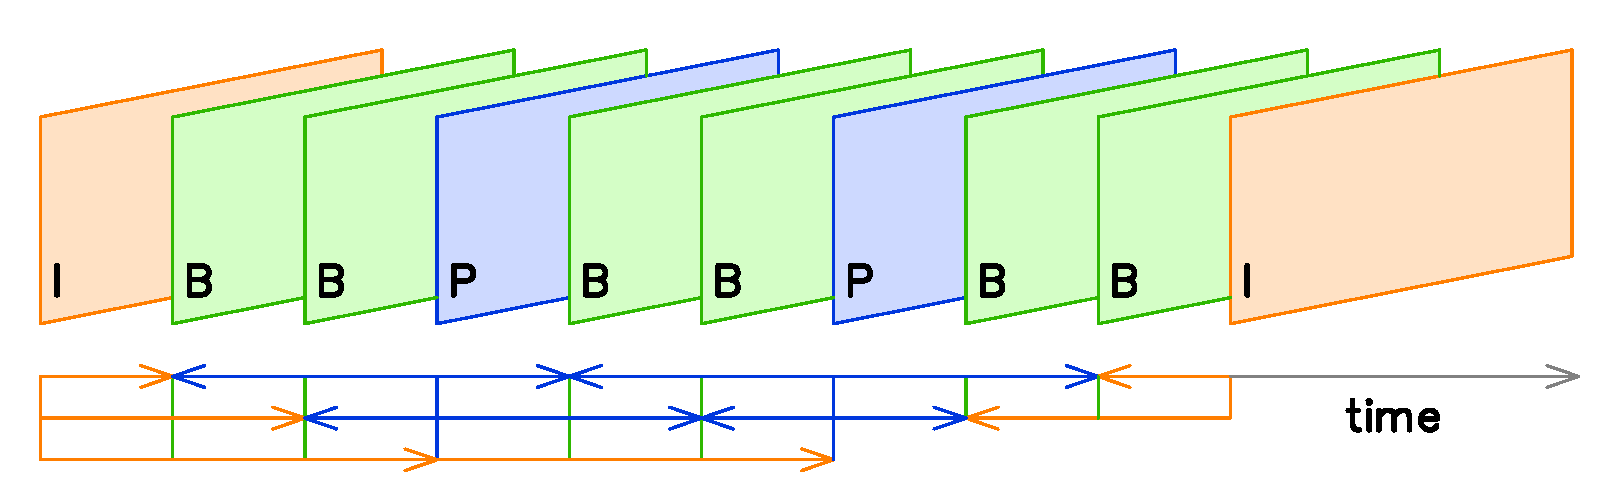
\includegraphics[width=0.7\textwidth, height=0.7\textheight, keepaspectratio]{img/IPB_images_sequence.png}}
\caption{An example of interleaved I-, B- and P-frames representing a video stream. The encoder may choose a different sequence of frame types. Figure reproduced from ``Inter frame'', Wikipedia~\cite{interframe-wiki}.}
\label{fig:ipb-seq}
\end{figure}

During encoding, a P-frame is partitioned into a grid of "\emph{macroblocks}" of 16x16 pixels\footnote{H.264 (the latest MPEG codec) allows higher granularity for fine details by allowing some blocks to be 8x8, 8x16 or 16x8.}. For each macroblock, the encoder searches for its most similar match in the predecessor frame within a spatially bounded region (search window)~\cite[p.~256]{richardson2004h}. The difference in pixels between the matched block and the original is called the \emph{prediction error}, and the displacement between the two is called the \emph{motion vector} (Figure~\ref{fig:mb-search}). We can say that a block of pixels has moved since the predecessor frame by the amount specified by its motion vector and, in addition to motion, pixels themselves have changed according to the prediction error.

\begin{figure}[tbh]
\centerline{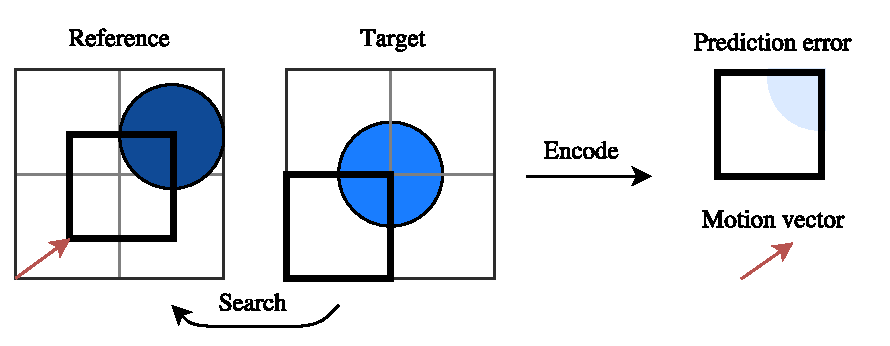
\includegraphics[width=0.7\textwidth,height=0.7\textheight,keepaspectratio]
{img/macroblock-diagram.pdf}}
\caption{An illustration of a macroblock search from the current (target) frame to the predecessor (reference) frame. A macroblock is encoded using its prediction error and  motion vector.}
\label{fig:mb-search}
\end{figure} 

\subsection{Motion vectors as embedding space}
\label{mv-emb-space}

This project considers the least-significant-bit (LSB) steganography: a technique that exploits the fact that in the binary representation of a value the LSB typically corresponds to the highest granularity level, so changes to the LSB are less likely to produce a noticeable difference in the output~\cite{bateman}.

Computing motion vectors is a tradeoff between accuracy and computation time, tuned using the search window size. This means that codecs typically don't find a globally optimal motion vector, resulting in a non-minimal prediction error~\cite[p.~257]{richardson2004h}. Since this means a non-minimal prediction error is not unusual, applying LSB steganography to a motion vector (which would lead to a small prediction error change to preserve output integrity) is less likely to be noticed.

To estimate the embedding capacity, we generalise how all implemented embedding schemes should operate on motion vectors. Suppose an embedding scheme processes every motion vector in a grid individually for every frame and has an associated selection function $f$ which provides a number of bits that can be embedded into a particular motion vector. Later on, this function will allow to conveniently define a MV selection criteria for different embedding schemes.

\begin{definition}{Embedding capacity for video}

Let $M$ be an embedding scheme with an associated function $f_M : \mathbb{R}^2 \rightarrow \mathbb{N}$, which calculates how many bits can be embedded into a particular motion vector $\overrightarrow{mv} \in \mathbb{R}^2$. Then for an MPEG-encoded video $V$, the embedding capacity $\mathcal{C}_{V, M}$ is defined as:

$$ \mathcal{C}_{V, M} = \sum_{p \in \text{P-frames}(V)} \: \sum^{H}_{j = 0} \sum^{W}_{i = 0} f_M(\overrightarrow{mv}^p_{i, j})$$

where $W$ and $H$ are width and height of the macroblock grid, P-frames$(V)$ is a set of all P-frames of a video $V$ and $\overrightarrow{mv}^p_{i, j}$ is the MV of a macroblock  in $i$-th row and $j$-th column of the frame $p$.

\end{definition}

To see whether videos could hold a non-negligible amount of hidden data, one can estimate $\mathcal{C}_{V, M}$ by taking a product of the number of P-frames, the total number of MVs per frame and the average number of bits embedded per MV. For instance, an average HD video could reasonably have 6--15 P-frames per second\footnote{Depends on how often the encoder decides to use B-frames and I-frames. P-frames are better for video streaming as they do not require the successor frame during decoding.} with 3600 MVs each\footnote{If video's resolution is 1280x720 (HD), 16x16 macroblocks would partition the frame into a grid of size 80x45. This gives 3600 macroblocks in total.}. Assuming only a quarter of each frame would contain embedded data, I estimate the channel's capacity to be 5.4--13 Kbits/s, which is sufficient to hold meaningfully-sized payloads. 

\section{Requirements analysis}

The project has two main software deliverables:
\begin{itemize}
\item  An application that allows a user to embed secret messages into MPEG video files using a selection of LSB embedding algorithms.
\item A steganalysis suite that implements some general-purpose routines to detect motion vector-based steganography.
\end{itemize}

Below is a list of requirements for both deliverables, prioritised using \emph{MoSCoW} criteria~\cite{softid-notes}.

\subsection{Steganographic application}
\label{req-steg-app}
\begin{itemize}
\item (M) Ability to access motion vectors of an MPEG video file.
\item (M) Ability to reliably embed data within motion vectors.
\item (M) Multiple LSB embedding techniques.
\item (M) User-friendly (CLI) binaries to perform embedding and extraction.
\item (S) Encryption of the secret message prior to embedding.
\item (S) Integration with an existing video codec.
\end{itemize}

\subsection{Steganalysis suite}
\label{req-steg-suite}
\begin{itemize}
\item (M) Ability to extract and process motion vector data.
\item (M) Multiple steganalysis methods.
\item (M) Documentation on usage and interpretation of the results.
\item (M) Evident effectiveness in detecting implemented embedding techniques.
\item (S) Compatibility with existing scientific computation packages (Matlab or Python-based packages)
\item (S) Usefulness (verbosity, amount of information provided) to the steganalyst.
\end{itemize}

\section{Project workflow}

\subsection{Technical choices}
\label{tech-choices}

The steganographic application requires modifying MPEG video files, which in turn requires parsing the format of a file, modifying motion vector values, and repackaging the data back into a playable video. Developing a codec does not relate to steganography and is potentially error-prone, so I leverage an existing set of codecs---\texttt{FFmpeg}\footnote{\url{https://www.ffmpeg.org/}}---to achieve this. As codecs are typically written in C or C++, it is a natural choice for this task to and makes the integration easier.

Performing encryption prior to embedding requires using a cryptographic library. I chose \emph{Crypto++}, a popular C++ cryptography library.

The steganalysis suite was integrated into the \emph{Matlab} scientific computation package for user's benefit, because it provides useful tools, such as statistical primitives, plotting capabilities and classifiers, without changing the environment. I chose Matlab because of its widespread use and comprehensive functionality.

\subsection{Risk analysis}
FFmpeg is a complex piece of software, mostly written in a style of C that sacrifices clarity for performance. A potential risk for the project was the difficulty of proper integration with FFmpeg and hence inability to access or reliably modify motion vectors. Complete failure to do so was unlikely, but it could have consumed a significant amount of development time. To mitigate this, some ``catch-up'' time was allocated in the project timetable.   

\subsection{Development choices}
\begin{itemize}
\item \emph{Git} was used for version control, allowing quick roll-back and managing multiple source trees using branches.
\item \emph{Backups} were done by uploading the source tree and other relevant files to Dropbox. The git repository itself was hosted remotely on GitHub.
\item \emph{Testing} was done both manually and using unit tests to verify that software performs as intended. Unit tests were implemented using the Google Test framework. As a good practice, compiler warnings were treated as errors. 
\item \emph{The iterative (spiral) development model} was used, which allowed continuously adding and testing new embedding schemes and steganalysis methods.
\item I aimed for \emph{modular design} of software components thoughout the development, which enabled better maintainability and testability, and well-defined interfaces allowed changing internal implementation without breaking compatibility with other components.
\end{itemize}

\section{Starting point}
This project uses some cryptography concepts introduced in the Part IB \textit{Security I} course. I have some C++ knowledge from past programming experience and the \textit{Programming in C and C++} course. 

Prior to submitting the proposal, I familiarised myself with the basic concepts of steganography and LSB embedding though some introductory texts and relevant papers, and looked at the H.264 codec format.

During the development of this project I made use of material covered in the following Part II courses:
\begin{itemize}
\item \textit{Information Theory} --- channel capacity, error correcting codes;
\item \textit{\LaTeX~and Matlab} --- typesetting and basics of Matlab;
\item \textit{Artificial Intelligence II} --- classifier evaluation.
\end{itemize}

\bigskip
\subsubsection*{Summary}
This chapter summarised the theoretical and practical background necessary to start the implementation. The next chapter will cover the design and features of the system, implemented steganographic algorithms and steganalysis methods, together with some in-line evaluation.

% Implementation
\cleardoublepage
\chapter{Implementation}

\textit{This chapter covers the implementation details for the steganographic application and the steganalysis suite. I discuss the operation of the encoder and decoder applications, integration with the codec, structure and implementation of the embedding algorithms, and the details of some steganalytic attacks. Some in-line evaluation of algorithms is presented to motivate the design improvements.}

\section{Steganographic application}

\subsection{Integration with FFmpeg}
\label{integrate-ffmpeg}

As discussed in section \ref{tech-choices}, FFmpeg is used to modify MPEG videos. Finding a suitable way to integrate with FFmpeg was one of the biggest challenges encountered early on. FFmpeg comprises several smaller libraries, each responsible for tasks such as stream multiplexing, resampling, or supporting I/O devices. The most suitable library for my purposes with was \texttt{libavcodec} which implements various audio and video codecs. Due to its popularity, I decided to focus on the H.264 codec, which FFmpeg offloads to a separate library: \texttt{libx264}. Although \texttt{libavcodec} exposes an API for interacting with its codecs, this API provides no way to manipulate motion vectors. As such, \texttt{libavcodec} needed modifying to either introduce an additional API or to have it call my steganographic routines itself.

Initially, I looked for a point in the macroblock search phase where motion vectors would already be available, but the prediction error would not have been computed yet. This would allow modification of MVs without the need to also update the prediction error to preserve the video output. Unfortunately, since both FFmpeg and \texttt{libx264} exhibit complex data flow, and are written in optimised C, analysis proved more difficult than anticipated, delaying the project by four weeks compared to the initial timeline. The plan was then changed to:
\begin{itemize}
\item Use a codec contained within \texttt{libavcodec}, obviating the need to touch \texttt{libx264}. I chose MPEG-4 Part 2 (\texttt{xvid}), H.264's popular predecessor.
\item Focus on modifying motion vectors, because it is essential to the project. The macroblock search is deep within the encoding pipeline, making it less amenable to modification. Instead, I chose to modify motion vectors before they are written to the output file.
\end{itemize}

Unfortunately, changing the motion vectors so late in the process means the prediction error has been calculated for the original motion vector, not the modified one. This means the steganography will (very slightly) alter the result of decoding the video. An experiment on human subjects was conducted to determine if this visual footprint is noticeable. This is further discussed in section \ref{exp-human-subj}.

\subsection{Steganography library}

\subsubsection{C API}

To achieve a modular design and decouple from FFmpeg, the implemented steganographic algorithms were separated into a standalone library \texttt{movestlib}\footnote{\texttt{movest} (\underline{mo}tion \underline{ve}ctor \underline {st}eganography) is the codename for this project.}. The library is implemented in C++, exposing a C API for integration with the encoder and decoder applications, and FFmpeg (Figure \ref{fig:movest-c-api}). To simplify the integration, FFmpeg calls library methods directly. The exact operation of these methods is described in section \ref{enc-dec-bin} using the encoder and decoder as examples.

\begin{figure}[tbh]
\centering
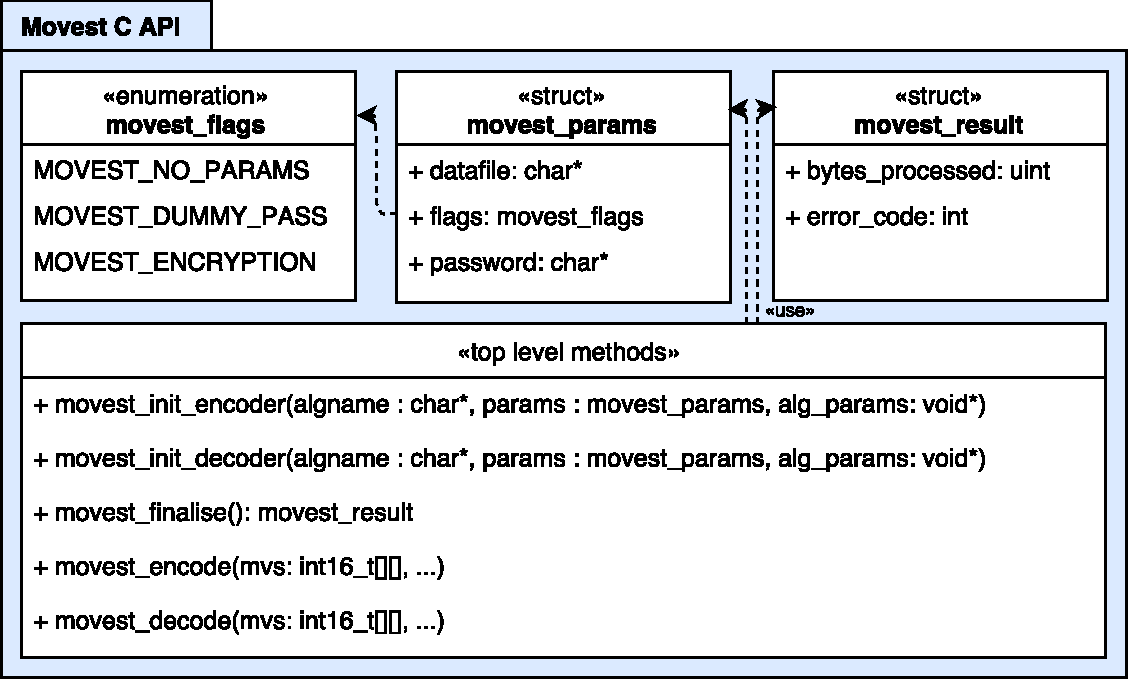
\includegraphics[width=0.9\textwidth]{img/movest_c_api.pdf}
\caption{UML diagram of the C API provided by \texttt{movestlib}. (Some method parameters omitted for brevity.)}
\label{fig:movest-c-api}
\end{figure}

A singleton instance of an embedding algorithm is kept active after initialisation. FFmpeg feeds motion vector data into the algorithm by calling C API methods \texttt{movest\_encode/decode}.  

\begin{figure}[!htbp]
\centering
\captionsetup{width=\textwidth}
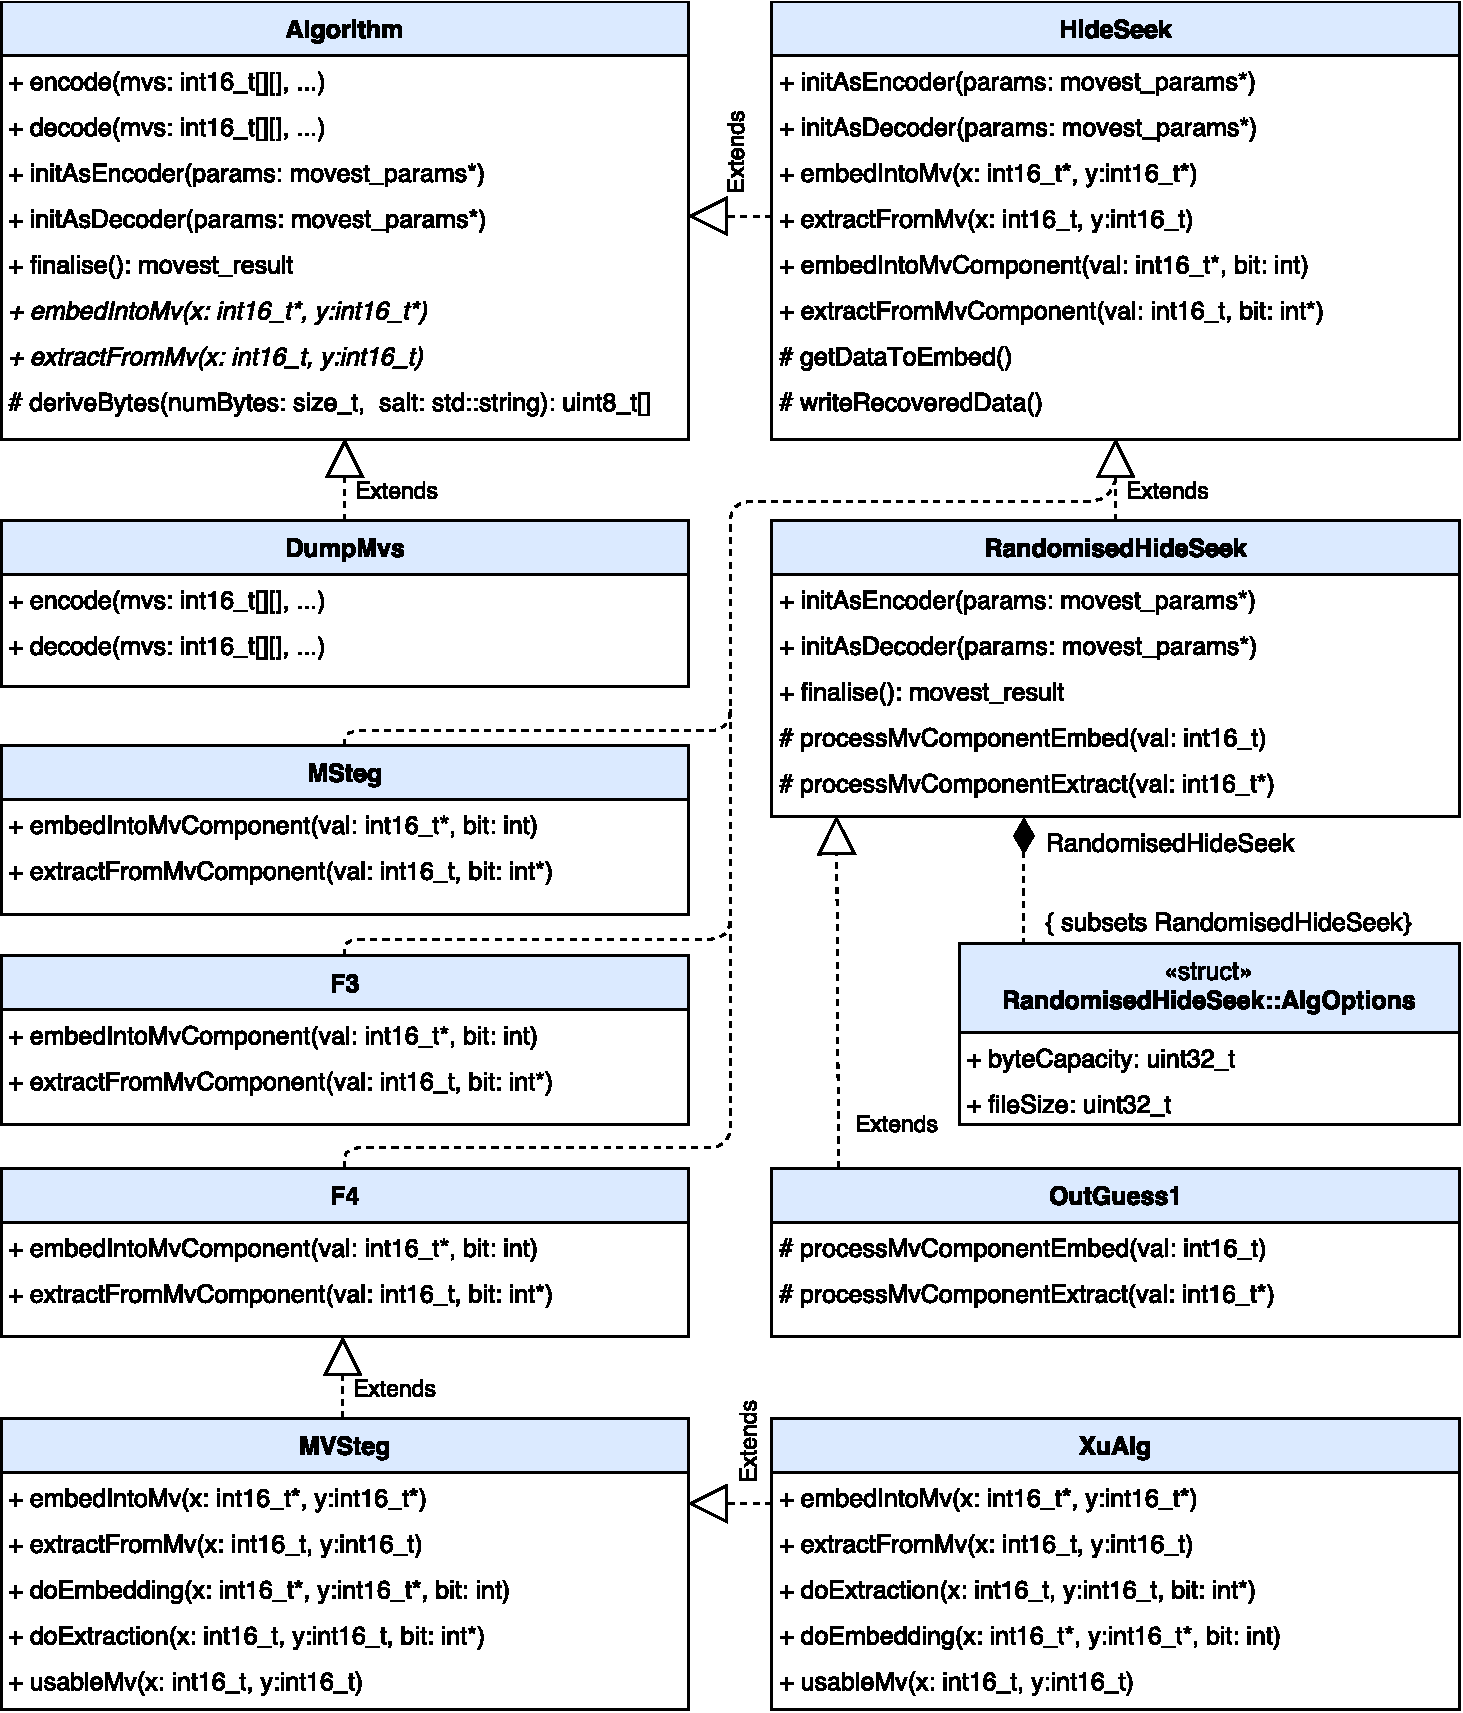
\includegraphics[width=\textwidth]{img/movest_alg_class_diag.pdf}
\caption{UML diagram of embedding algorithms implemented in \texttt{movestlib}. (Some unimportant fields, methods and method parameters omitted for brevity.)}
\label{fig:movest_alg_class_diag}
\end{figure}

\subsubsection{Class hierarchy}

To encourage modularity and code reuse, the embedding algorithms were implemented as OOP classes. The class hierarchy is presented in Figure \ref{fig:movest_alg_class_diag}. \texttt{Algorithm} is the base class for all embedding algorithms, containing common functionality such as initialising the payload file or operating on every motion vector of a suitable type. Most algorithms, however, extend \texttt{HideSeek} or its subclasses to benefit from the following more specific functionality:

\begin{itemize}
\item Operating on a per-component basis. Motion vectors are stored as $x$ and $y$ components and many algorithms treat them independently (\texttt{RandomisedHideSeek, OutGuess1}).
\item Sequential data fetching and stopping criteria. Some algorithms read and embed payload bits sequentially and require knowledge of when to stop embedding (\texttt{XuAlg, MVSteg}).
\item Both of above (\texttt{MSteg, F3, F4}).
\end{itemize}

\subsubsection{Encryption}
\label{encryption}
Encrypting the payload hides the structure of the data by making it indistinguishable from random noise. This makes it hard to detect in already-noisy regions of the cover, as well as causing it to remain unreadable by an adversary even if the steganography was broken. \texttt{movestlib} achieves this by implementing a proxy object for accessing the payload, and encrypting or decrypting the data on the fly (\texttt{MOVEST\_ENCRYPTION} flag). Encryption is done using AES in counter (CTR) mode with a 256-bit key, using the Crypto++ library (since implementing your own cryptography primitives is time consuming and error prone). The key and the initialisation vector are derived from the user-supplied password using the industry-standard PBKDF2-HMAC-SHA1 key derivation function~\cite{kaliski2000rfc}.

\subsection{Encoder and decoder applications}
\label{enc-dec-bin}
The project provides video-processing applications for embedding and recovering the payload from a video file. They are largely based on FFmpeg examples for transcoding (\texttt{transcoding.c}) and motion vector extraction (\texttt{extract\_mvs.c}), which already contain the code to trigger code paths in FFmpeg that I have modified. Figure \ref{fig:encoder-help} provides an example of options available for the embedding application (encoder).

Before letting FFmpeg process the video, applications parse user input to initialise \texttt{movestlib} with required data, such as the embedding algorithm, the payload file path, and the encryption password (\texttt{movest\_init\_encoder/decoder}). Some of the steganography algorithms need to determine global properties---such as the embedding capacity---of the video in order to operate on it. Since FFmpeg processes the video as a stream, historical frames are not available, and making it behave otherwise would involve storing the entire video stream in memory. So, the encoder performs a dry run (\texttt{MOVEST\_DUMMY\_PASS} flag) to compute global video properties, before running a second pass to perform the actual embedding.

\begin{figure}[tbh]
\vspace{1em}
\centering
\begin{minipage}{0.9\textwidth}
\begingroup
    \fontsize{10pt}{12pt}\selectfont
\begin{alltt}
MOVEST Encoder, (c) 2016
Usage: movest_enc -a <algorithm> -d <data_file> [--encrypt, -p <password>]
<input_video> <output_video>

Command line arguments:
 --encrypt        Perform encryption of the data prior to embedding
 -a/--algorithm   An embedding algorithm to use
 -d/--data        Path to a file, containing the payload
 -p/--password    An encryption password to use
 -h/--help        Print this help message

Available algorithm options:
 'dummypass' (does not embed data)
 'hidenseek' 'msteg' 'f3' 'f4'
 'mvsteg' 'xualg'
 'rand-hidenseek' 'outguess1'
\end{alltt}
\endgroup
\end{minipage}
\caption{User help (\texttt{-{}-help}) of the Movest encoder.}
\label{fig:encoder-help}
\end{figure}

\section{Steganalysis techniques}
\label{steg-tech}

The steganalysis techniques for this project were implemented in Matlab, where the large library of pre-existing statistical and data processing routines makes things considerably simpler.

\subsection{Motion vector import}
\label{mv-import}

The Movest decoder can be configured to dump the motion vector components in a human-readable text format that can later be imported to Matlab as a 3D matrix (\texttt{loadmvs.m}) in which the element at $(i, j, k)$ refers to a macroblock at $i$-th row, $j$-th column of the $k$-th frame. 

FFmpeg may choose to omit some macroblocks to save space by marking them as ``skipped'', causing the decoder to infer the motion from neighbouring blocks~\cite{tourapis2004direct}. For the sake of completeness of the macroblock grid, FFmpeg reports an MV of $(0, 0)$ for a skip macroblock. The Movest decoder stores metadata for such macroblocks allowing them to be ignored during later processing (\texttt{typedmvs.m}).

\subsection{LSB plane, 2D plotting and aggregation into bytes}

Since this project implements LSB steganography, the suite includes a function (\texttt{lsbplane.m}) to project least significant bits out of every motion vector component value. If the embedding algorithm sets the LSBs of motion vectors to exactly payload bits, LSBs can be immediately subjected to visual analysis to reveal any patterns in the data. This is best illustrated by an example.

\begin{figure}[tbh]
\centerline{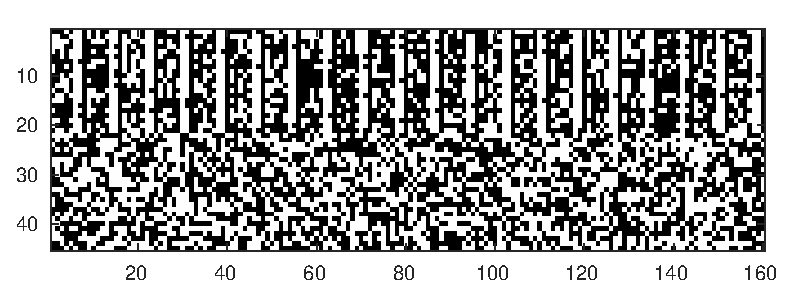
\includegraphics{img/unencrypted-enc.eps}}
\caption{Sample output of \texttt{plot2d} over LSB plane. Even-numbered and odd-numbered columns contain LSBs for $x$ and $y$ components respectively.}
\label{fig:unencrypted-enc}
\end{figure}

Figure \ref{fig:unencrypted-enc} shows an example of a 2-valued heatmap (\texttt{plot2d.m}) produced by the suite. The plot shows a clear pattern of embedded data in the first half of the frame. Given that there are repeating columns of 1s every 8 bits, a steganalyst could make an educated guess that the payload is ASCII-encoded and attempt to group bits into bytes to reproduce the text (\texttt{aggregateIntoBytes.m}):

\begin{alltt}
    >> char\footnote{In Matlab, \texttt{char} interprets an integer value as an ASCII-encoded character.}(aggregateIntoBytes(mvs, types))'
    ans = hello world\ldots
\end{alltt}

\subsection{Histogram and $\chi^2$ (Chi-Squared) attack}
\label{hist-chisq-attack}

The distribution of motion vectors can be visualised using a histogram (\texttt{mvhist.m}). This can be a useful source of information for a steganalyst because peculiarities in the histogram can reveal that motion vectors have been modified. MV histograms typically have a sharp peak at 0 and exponentially decay on both sides. Since these histograms are affected by the direction of motion in the video, decay rates may vary, and we may see additional peaks or plateaus (Figure \ref{fig:histogram-example}).

\begin{figure}[tbh]
\centerline{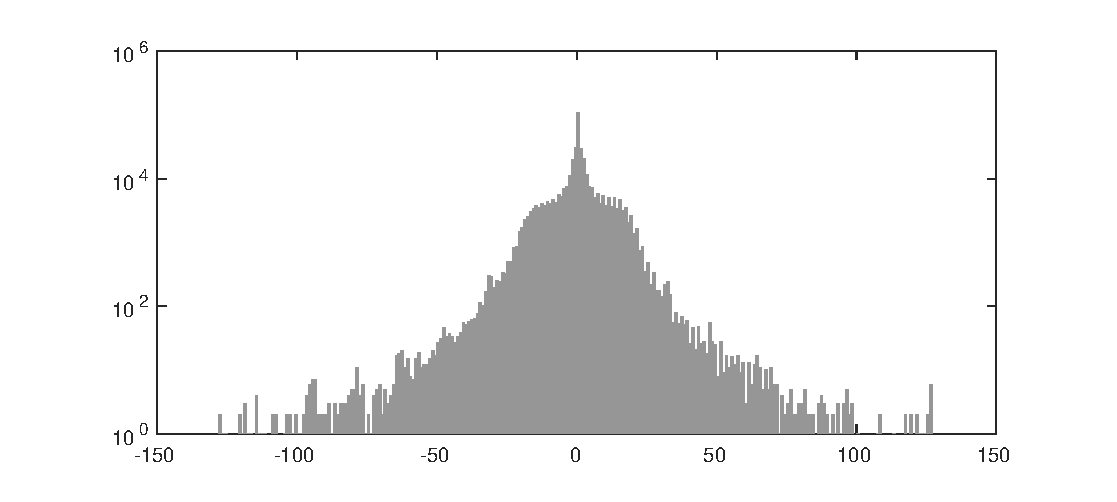
\includegraphics[scale=0.75]{img/histogram-example.eps}}
\caption{Sample output of \texttt{mvhist} for the $x$ component of all motion vectors in a non-stego video.}
\label{fig:histogram-example}
\end{figure}

Westfeld and Pfitzmann~\cite{westfeld1999attacks} developed a method for attacking image steganography called the \emph{$\chi^2$ attack}, which can also be applied to motion vectors. They hypothesise that, due to the nature of JPEG DCT coefficients (to which the method was originally applied), it is unlikely that adjacent histogram bars will be the same height. The variability of motion vector data suggests that this property also applies to motion vectors.

Since the encrypted payload will, on average, have the same number of 0 and 1 bits, so will the LSBs of motion vector values. Therefore, values in each even-odd pair (pair of values that only differs in the LSB: 0 and 1, 2 and 3, 4 and 5, \emph{etc.}) should occur the same number of times, and their corresponding histogram bars should be of the same height.

We can now devise a statistical procedure (\texttt{chiSquareAttack.m}) for determining the probability that a given set of motion vectors contains a secret message. We consider even-odd pairs of values of the form $(2k, 2k+1)$. 

Let $X_k$ and $Y_k$ be the number of times values $2k$ and $2k+1$ occur as motion vector values, and their average, $Z_k = \frac{X_k + Y_k}{2}$. If the video contains a payload, $X_k$ and $Y_k$ should be almost equal and distributed as $Z_k$. To prevent influence from the noise in data, pairs that have $Z_k < 8$ are considered to be under-represented and are neglected in further analysis (\emph{minimum frequency condition}\footnote{The original paper specifies $Z_k < 2$, but I found that this threshold was too low for motion vector data.}).

We can use the \emph{$\chi^2$ (chi-square) test} to check the hypothesis that there is no significant difference between $X_k$ and $Z_k$ (null hypothesis). The case for $Y_k$ is symmetric and not considered further. The test tells us we can compute

$$ \chi^2_{n-1} \approx \sum^{n}_{k=0} \frac{(\text{observed}_k - \text{expected}_k)^2}{\text{expected}_k}= \sum^{255}_{k=-255} \frac{(X_k - Z_k)^2}{Z_k} $$ 

from which we can obtain the $p$-value of data supporting the null hypothesis. $1 - p$ is interpreted as the probability that the cover contains the payload~\cite{westfeld1999attacks}:

$$ \mathbb{P}\text{(stego-video)} = 1 - \frac{1}{2^{\frac{n-1}{2}}\Gamma(\frac{n-1}{2})}\int_0^{\chi^2_{n-1}}t^{\frac{n-1}{2}−1}e^{-t/2}dt $$  

This method can also estimate the size of the payload. We can see from the expression for $\chi^2_{n-1}$ that it is sensitive to small changes: the value stays close to 0 when data contains the payload ($X_k - Z_k \approx 0$) and is big otherwise. We can iteratively build up the histogram and update $\chi^2_{n-1}$ as data for every frame comes in. We know that when the value starts increasing (and probability decreases), the data no longer contains the payload, so we can put a bound on the payload size. 

\subsection{Reversion technique}
\label{rev-tech-theory}
Cao \emph{et al.}~\cite{cao2012video} proved that, in general, since transcoding a video causes a new motion vector search to be performed, it tends to revert motion vectors to their original values, destroying the payload. Measuring this change can expose the embedding: if a video contains a payload, we expect the differences between pre- and post-transcoding motion vectors to be high.

\begin{wrapfigure}[13]{R}{6cm}
\vspace{-15pt}
\centering
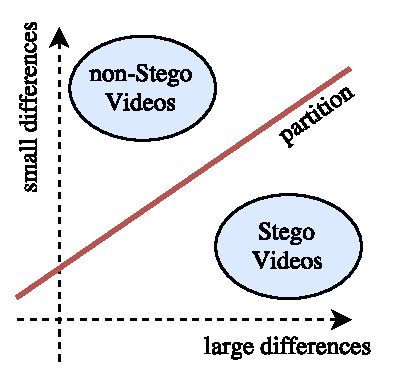
\includegraphics[width=5.5cm]{img/movest_reversion_sketch.pdf}
\caption{Partitioning stego and non-stego videos.}
\label{fig:movest-reversion-sketch}
\end{wrapfigure}

\emph{Sum of absolute differences (SAD)} is used to compute the difference between respective components of motion vectors:

$$ \Delta \overrightarrow{mv^p_{ij}} = |(\overrightarrow{o^p_{ij}})_x - (\overrightarrow{t^p_{ij}})_x| +  |(\overrightarrow{o^p_{ij}})_y - (\overrightarrow{t^p_{ij}})_y|$$

where $\overrightarrow{o^p_{ij}}$ and $\overrightarrow{t^p_{ij}}$ are motion vectors of the original and transcoded video. To determine how common small and large differences are in a video, the algorithm computes a normalised vector of frequencies for every value of $\Delta\overrightarrow{mv^p_{ij}}$. The $k$-th element of the vector gives the proportion of $\Delta\overrightarrow{mv^p_{ij}} = k$ occurring among all SADs.

The reversion hypothesis suggests this approach for distinguishing between a stego summarised in Figure \ref{fig:movest-reversion-sketch}: stego videos will have a lower frequency of small differences ($\Delta\overrightarrow{mv^p_{ij}} < 2$), but a higher frequency of larger differences ($\Delta\overrightarrow{mv^p_{ij}} \geq 2$) than non-stego videos.

A classifier can be built to attempt to differentiate between these two classes of video. I decided to use a Support Vector Machine (SVM)\footnote{\url{http://uk.mathworks.com/help/stats/support-vector-machines-for-binary-classification.html}} with a linear kernel (as Figure \ref{fig:movest-reversion-sketch} suggests), trained using Matlab's \texttt{fitcsvm} routine. Evaluation of this method is presented in section \ref{rev-tech}.

\section{Embedding algorithms}
\label{emb-alg}

This section presents the 8 LSB steganography algorithms implemented by this project.

\subsection{Hide \& Seek}
\label{hide-n-seek}

\emph{Hide \& Seek}~\cite{bateman} embeds payload bits into both $x$ and $y$ components of each motion vector by setting their LSB to that of the payload. This achieves the maximal capacity of 2 bits per macroblock for an LSB scheme, but is susceptible to all the attacks described in the previous section.

\begin{figure}[tbh]
\centerline{
\begin{subfigure}[t]{0.4\textwidth}
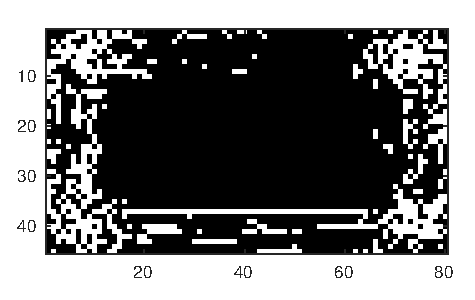
\includegraphics[scale=0.8]{img/pre-lsb-embedding.eps}
\end{subfigure}
~
\begin{subfigure}[t]{0.4\textwidth}
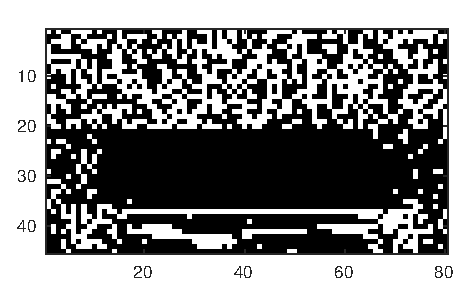
\includegraphics[scale=0.8]{img/post-lsb-embedding.eps}
\end{subfigure}
}
\caption{An example of a frame prior to embedding (left) and after embedding at 45\% capacity (right).}
\label{fig:visual-analysis-example}
\end{figure}

Since data is embedded into all possible macroblocks, visual analysis allows easy detection in non-noisy regions. This is illustrated in Figure \ref{fig:visual-analysis-example}: unusual noise in the first half of the frame exposes the embedding. 

\subsection{MSteg}
\label{msteg}

\emph{MSteg} is my straightforward adaptation of the \emph{JSteg} algorithm~\cite{bateman}, which was initially developed for embedding into JPEG DCT coefficients. The algorithm operates in the same way as Hide \& Seek, but addresses the visual detection problem by not embedding into ``still'' regions, where noise would be easily detectable. Specifically, it avoids embedding bits into 0-valued motion vector components. Components with value 1 are also avoided, since embedding bit 0 would turn them into zeros, making decoding ambiguous.

Figure \ref{fig:msteg-visual} shows that MSteg performs better when subjected to visual analysis. However, it is susceptible to the $\chi^2$ attack as it causes values in even-odd pairs to occur with the same frequency (see Section \ref{hist-chisq-attack} and Figure \ref{fig:chisq-attack} below), as shown by the histogram in Figure \ref{fig:msteg-hist}.

\begin{figure}[tbh]
\centering
\begin{minipage}[t]{.4\textwidth}
  \centering
  \captionsetup{width=\textwidth}
  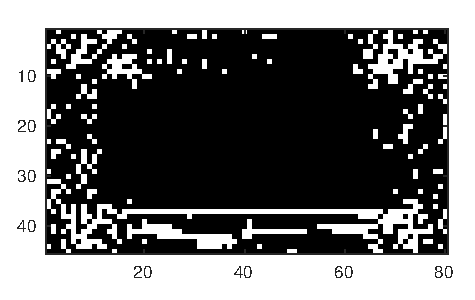
\includegraphics[scale=0.8]{img/msteg-visual.eps}
  \caption{LSB plane of the frame subjected to MSteg embedding.}
  \label{fig:msteg-visual}
\end{minipage}
\quad\quad
\begin{minipage}[t]{.45\textwidth}
  \centering
  \captionsetup{width=\textwidth}
  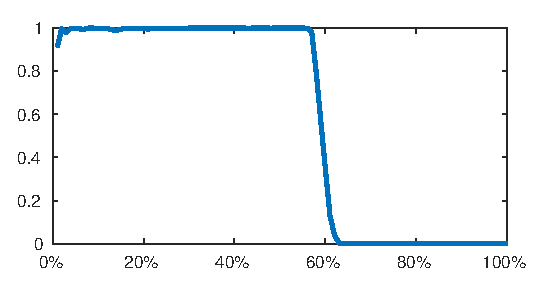
\includegraphics[scale=0.84]{img/chisq-attack.eps}
  \caption{An example of probability of embedding computed by the $\chi^2$ attack when embedding was done at 58\% of capacity.}
  \label{fig:chisq-attack}
\end{minipage}
\end{figure}

\begin{figure}[tbh]
\centering
\resizebox{0.6\textwidth}{!}{%LaTeX with PSTricks extensions
%%Creator: inkscape 0.91
%%Please note this file requires PSTricks extensions
\psset{xunit=.5pt,yunit=.5pt,runit=.5pt}
\begin{pspicture}(349,154)
{
\newrgbcolor{curcolor}{1 1 1}
\pscustom[linestyle=none,fillstyle=solid,fillcolor=curcolor]
{
\newpath
\moveto(0,154)
\lineto(349,154)
\lineto(349,0)
\lineto(0,0)
\closepath
}
}
{
\newrgbcolor{curcolor}{1 1 1}
\pscustom[linestyle=none,fillstyle=solid,fillcolor=curcolor]
{
\newpath
\moveto(0,154)
\lineto(349,154)
\lineto(349,0)
\lineto(0,0)
\closepath
}
}
{
\newrgbcolor{curcolor}{1 1 1}
\pscustom[linestyle=none,fillstyle=solid,fillcolor=curcolor]
{
\newpath
\moveto(25,20)
\lineto(349,20)
\lineto(349,138)
\lineto(25,138)
\closepath
}
}
{
\newrgbcolor{curcolor}{0.14901961 0.14901961 0.14901961}
\pscustom[linewidth=0.66670001,linecolor=curcolor]
{
\newpath
\moveto(25,20)
\lineto(349,20)
}
}
{
\newrgbcolor{curcolor}{0.14901961 0.14901961 0.14901961}
\pscustom[linewidth=0.66670001,linecolor=curcolor]
{
\newpath
\moveto(25,138)
\lineto(349,138)
}
}
{
\newrgbcolor{curcolor}{0.14901961 0.14901961 0.14901961}
\pscustom[linewidth=0.66670001,linecolor=curcolor]
{
\newpath
\moveto(39.72729874,20)
\lineto(39.72729874,23.24000549)
}
}
{
\newrgbcolor{curcolor}{0.14901961 0.14901961 0.14901961}
\pscustom[linewidth=0.66670001,linecolor=curcolor]
{
\newpath
\moveto(113.36360168,20)
\lineto(113.36360168,23.24000549)
}
}
{
\newrgbcolor{curcolor}{0.14901961 0.14901961 0.14901961}
\pscustom[linewidth=0.66670001,linecolor=curcolor]
{
\newpath
\moveto(187,20)
\lineto(187,23.24000549)
}
}
{
\newrgbcolor{curcolor}{0.14901961 0.14901961 0.14901961}
\pscustom[linewidth=0.66670001,linecolor=curcolor]
{
\newpath
\moveto(260.63641357,20)
\lineto(260.63641357,23.24000549)
}
}
{
\newrgbcolor{curcolor}{0.14901961 0.14901961 0.14901961}
\pscustom[linewidth=0.66670001,linecolor=curcolor]
{
\newpath
\moveto(334.27270508,20)
\lineto(334.27270508,23.24000549)
}
}
{
\newrgbcolor{curcolor}{0.14901961 0.14901961 0.14901961}
\pscustom[linewidth=0.66670001,linecolor=curcolor]
{
\newpath
\moveto(39.72729874,138)
\lineto(39.72729874,134.76000023)
}
}
{
\newrgbcolor{curcolor}{0.14901961 0.14901961 0.14901961}
\pscustom[linewidth=0.66670001,linecolor=curcolor]
{
\newpath
\moveto(113.36360168,138)
\lineto(113.36360168,134.76000023)
}
}
{
\newrgbcolor{curcolor}{0.14901961 0.14901961 0.14901961}
\pscustom[linewidth=0.66670001,linecolor=curcolor]
{
\newpath
\moveto(187,138)
\lineto(187,134.76000023)
}
}
{
\newrgbcolor{curcolor}{0.14901961 0.14901961 0.14901961}
\pscustom[linewidth=0.66670001,linecolor=curcolor]
{
\newpath
\moveto(260.63641357,138)
\lineto(260.63641357,134.76000023)
}
}
{
\newrgbcolor{curcolor}{0.14901961 0.14901961 0.14901961}
\pscustom[linewidth=0.66670001,linecolor=curcolor]
{
\newpath
\moveto(334.27270508,138)
\lineto(334.27270508,134.76000023)
}
}
{
\newrgbcolor{curcolor}{0.14901961 0.14901961 0.14901961}
\pscustom[linestyle=none,fillstyle=solid,fillcolor=curcolor]
{
\newpath
\moveto(30.3132375,6.79057812)
\lineto(33.47144062,6.79057812)
\lineto(33.47144062,5.82964062)
\lineto(30.3132375,5.82964062)
\lineto(30.3132375,6.79057812)
\closepath
}
}
{
\newrgbcolor{curcolor}{0.14901961 0.14901961 0.14901961}
\pscustom[linestyle=none,fillstyle=solid,fillcolor=curcolor]
{
\newpath
\moveto(36.36597187,4.01909375)
\lineto(40.49683125,4.01909375)
\lineto(40.49683125,3.023)
\lineto(34.94214375,3.023)
\lineto(34.94214375,4.01909375)
\curveto(35.3913625,4.4839375)(36.00269062,5.10698437)(36.77612812,5.88823437)
\curveto(37.55347187,6.67339062)(38.04175312,7.17925)(38.24097187,7.4058125)
\curveto(38.61987812,7.83159375)(38.88355,8.19096875)(39.0319875,8.4839375)
\curveto(39.18433125,8.7808125)(39.26050312,9.07182812)(39.26050312,9.35698437)
\curveto(39.26050312,9.82182812)(39.09644062,10.20073437)(38.76831562,10.49370312)
\curveto(38.44409687,10.78667187)(38.02026875,10.93315625)(37.49683125,10.93315625)
\curveto(37.1257375,10.93315625)(36.73315937,10.86870312)(36.31909687,10.73979687)
\curveto(35.90894062,10.61089062)(35.4694875,10.41557812)(35.0007375,10.15385937)
\lineto(35.0007375,11.34917187)
\curveto(35.4773,11.54057812)(35.9226125,11.68510937)(36.336675,11.78276562)
\curveto(36.7507375,11.88042187)(37.12964375,11.92925)(37.47339375,11.92925)
\curveto(38.37964375,11.92925)(39.1023,11.7026875)(39.6413625,11.2495625)
\curveto(40.180425,10.7964375)(40.44995625,10.19096875)(40.44995625,9.43315625)
\curveto(40.44995625,9.07378125)(40.38159687,8.73198437)(40.24487812,8.40776562)
\curveto(40.11206562,8.08745312)(39.867925,7.70854687)(39.51245625,7.27104687)
\curveto(39.4148,7.15776562)(39.10425312,6.82964062)(38.58081562,6.28667187)
\curveto(38.05737812,5.74760937)(37.31909687,4.99175)(36.36597187,4.01909375)
\closepath
}
}
{
\newrgbcolor{curcolor}{0.14901961 0.14901961 0.14901961}
\pscustom[linestyle=none,fillstyle=solid,fillcolor=curcolor]
{
\newpath
\moveto(45.51831562,10.99175)
\curveto(44.90894062,10.99175)(44.44995625,10.69096875)(44.1413625,10.08940625)
\curveto(43.836675,9.49175)(43.68433125,8.59135937)(43.68433125,7.38823437)
\curveto(43.68433125,6.18901562)(43.836675,5.288625)(44.1413625,4.6870625)
\curveto(44.44995625,4.08940625)(44.90894062,3.79057812)(45.51831562,3.79057812)
\curveto(46.13159687,3.79057812)(46.59058125,4.08940625)(46.89526875,4.6870625)
\curveto(47.2038625,5.288625)(47.35815937,6.18901562)(47.35815937,7.38823437)
\curveto(47.35815937,8.59135937)(47.2038625,9.49175)(46.89526875,10.08940625)
\curveto(46.59058125,10.69096875)(46.13159687,10.99175)(45.51831562,10.99175)
\closepath
\moveto(45.51831562,11.92925)
\curveto(46.49878437,11.92925)(47.24683125,11.54057812)(47.76245625,10.76323437)
\curveto(48.2819875,9.98979687)(48.54175312,8.86479687)(48.54175312,7.38823437)
\curveto(48.54175312,5.91557812)(48.2819875,4.79057812)(47.76245625,4.01323437)
\curveto(47.24683125,3.23979687)(46.49878437,2.85307812)(45.51831562,2.85307812)
\curveto(44.53784687,2.85307812)(43.78784687,3.23979687)(43.26831562,4.01323437)
\curveto(42.75269062,4.79057812)(42.49487812,5.91557812)(42.49487812,7.38823437)
\curveto(42.49487812,8.86479687)(42.75269062,9.98979687)(43.26831562,10.76323437)
\curveto(43.78784687,11.54057812)(44.53784687,11.92925)(45.51831562,11.92925)
\closepath
}
}
{
\newrgbcolor{curcolor}{0.14901961 0.14901961 0.14901961}
\pscustom[linestyle=none,fillstyle=solid,fillcolor=curcolor]
{
\newpath
\moveto(103.9495375,6.79057812)
\lineto(107.10774063,6.79057812)
\lineto(107.10774063,5.82964062)
\lineto(103.9495375,5.82964062)
\lineto(103.9495375,6.79057812)
\closepath
}
}
{
\newrgbcolor{curcolor}{0.14901961 0.14901961 0.14901961}
\pscustom[linestyle=none,fillstyle=solid,fillcolor=curcolor]
{
\newpath
\moveto(109.18781875,4.01909375)
\lineto(111.1214125,4.01909375)
\lineto(111.1214125,10.69292187)
\lineto(109.01789688,10.27104687)
\lineto(109.01789688,11.34917187)
\lineto(111.10969375,11.77104687)
\lineto(112.2932875,11.77104687)
\lineto(112.2932875,4.01909375)
\lineto(114.22688125,4.01909375)
\lineto(114.22688125,3.023)
\lineto(109.18781875,3.023)
\lineto(109.18781875,4.01909375)
\closepath
}
}
{
\newrgbcolor{curcolor}{0.14901961 0.14901961 0.14901961}
\pscustom[linestyle=none,fillstyle=solid,fillcolor=curcolor]
{
\newpath
\moveto(119.15461563,10.99175)
\curveto(118.54524063,10.99175)(118.08625625,10.69096875)(117.7776625,10.08940625)
\curveto(117.472975,9.49175)(117.32063125,8.59135937)(117.32063125,7.38823437)
\curveto(117.32063125,6.18901562)(117.472975,5.288625)(117.7776625,4.6870625)
\curveto(118.08625625,4.08940625)(118.54524063,3.79057812)(119.15461563,3.79057812)
\curveto(119.76789688,3.79057812)(120.22688125,4.08940625)(120.53156875,4.6870625)
\curveto(120.8401625,5.288625)(120.99445938,6.18901562)(120.99445938,7.38823437)
\curveto(120.99445938,8.59135937)(120.8401625,9.49175)(120.53156875,10.08940625)
\curveto(120.22688125,10.69096875)(119.76789688,10.99175)(119.15461563,10.99175)
\closepath
\moveto(119.15461563,11.92925)
\curveto(120.13508438,11.92925)(120.88313125,11.54057812)(121.39875625,10.76323437)
\curveto(121.9182875,9.98979687)(122.17805313,8.86479687)(122.17805313,7.38823437)
\curveto(122.17805313,5.91557812)(121.9182875,4.79057812)(121.39875625,4.01323437)
\curveto(120.88313125,3.23979687)(120.13508438,2.85307812)(119.15461563,2.85307812)
\curveto(118.17414688,2.85307812)(117.42414688,3.23979687)(116.90461563,4.01323437)
\curveto(116.38899063,4.79057812)(116.13117813,5.91557812)(116.13117813,7.38823437)
\curveto(116.13117813,8.86479687)(116.38899063,9.98979687)(116.90461563,10.76323437)
\curveto(117.42414688,11.54057812)(118.17414688,11.92925)(119.15461563,11.92925)
\closepath
}
}
{
\newrgbcolor{curcolor}{0.14901961 0.14901961 0.14901961}
\pscustom[linestyle=none,fillstyle=solid,fillcolor=curcolor]
{
\newpath
\moveto(186.81445312,10.99175)
\curveto(186.20507812,10.99175)(185.74609375,10.69096875)(185.4375,10.08940625)
\curveto(185.1328125,9.49175)(184.98046875,8.59135937)(184.98046875,7.38823437)
\curveto(184.98046875,6.18901562)(185.1328125,5.288625)(185.4375,4.6870625)
\curveto(185.74609375,4.08940625)(186.20507812,3.79057812)(186.81445312,3.79057812)
\curveto(187.42773438,3.79057812)(187.88671875,4.08940625)(188.19140625,4.6870625)
\curveto(188.5,5.288625)(188.65429688,6.18901562)(188.65429688,7.38823437)
\curveto(188.65429688,8.59135937)(188.5,9.49175)(188.19140625,10.08940625)
\curveto(187.88671875,10.69096875)(187.42773438,10.99175)(186.81445312,10.99175)
\closepath
\moveto(186.81445312,11.92925)
\curveto(187.79492188,11.92925)(188.54296875,11.54057812)(189.05859375,10.76323437)
\curveto(189.578125,9.98979687)(189.83789062,8.86479687)(189.83789062,7.38823437)
\curveto(189.83789062,5.91557812)(189.578125,4.79057812)(189.05859375,4.01323437)
\curveto(188.54296875,3.23979687)(187.79492188,2.85307812)(186.81445312,2.85307812)
\curveto(185.83398438,2.85307812)(185.08398438,3.23979687)(184.56445312,4.01323437)
\curveto(184.04882812,4.79057812)(183.79101562,5.91557812)(183.79101562,7.38823437)
\curveto(183.79101562,8.86479687)(184.04882812,9.98979687)(184.56445312,10.76323437)
\curveto(185.08398438,11.54057812)(185.83398438,11.92925)(186.81445312,11.92925)
\closepath
}
}
{
\newrgbcolor{curcolor}{0.14901961 0.14901961 0.14901961}
\pscustom[linestyle=none,fillstyle=solid,fillcolor=curcolor]
{
\newpath
\moveto(254.12468125,4.01909375)
\lineto(256.058275,4.01909375)
\lineto(256.058275,10.69292187)
\lineto(253.95475937,10.27104687)
\lineto(253.95475937,11.34917187)
\lineto(256.04655625,11.77104687)
\lineto(257.23015,11.77104687)
\lineto(257.23015,4.01909375)
\lineto(259.16374375,4.01909375)
\lineto(259.16374375,3.023)
\lineto(254.12468125,3.023)
\lineto(254.12468125,4.01909375)
\closepath
}
}
{
\newrgbcolor{curcolor}{0.14901961 0.14901961 0.14901961}
\pscustom[linestyle=none,fillstyle=solid,fillcolor=curcolor]
{
\newpath
\moveto(264.09147812,10.99175)
\curveto(263.48210312,10.99175)(263.02311875,10.69096875)(262.714525,10.08940625)
\curveto(262.4098375,9.49175)(262.25749375,8.59135937)(262.25749375,7.38823437)
\curveto(262.25749375,6.18901562)(262.4098375,5.288625)(262.714525,4.6870625)
\curveto(263.02311875,4.08940625)(263.48210312,3.79057812)(264.09147812,3.79057812)
\curveto(264.70475937,3.79057812)(265.16374375,4.08940625)(265.46843125,4.6870625)
\curveto(265.777025,5.288625)(265.93132187,6.18901562)(265.93132187,7.38823437)
\curveto(265.93132187,8.59135937)(265.777025,9.49175)(265.46843125,10.08940625)
\curveto(265.16374375,10.69096875)(264.70475937,10.99175)(264.09147812,10.99175)
\closepath
\moveto(264.09147812,11.92925)
\curveto(265.07194687,11.92925)(265.81999375,11.54057812)(266.33561875,10.76323437)
\curveto(266.85515,9.98979687)(267.11491562,8.86479687)(267.11491562,7.38823437)
\curveto(267.11491562,5.91557812)(266.85515,4.79057812)(266.33561875,4.01323437)
\curveto(265.81999375,3.23979687)(265.07194687,2.85307812)(264.09147812,2.85307812)
\curveto(263.11100937,2.85307812)(262.36100937,3.23979687)(261.84147812,4.01323437)
\curveto(261.32585312,4.79057812)(261.06804062,5.91557812)(261.06804062,7.38823437)
\curveto(261.06804062,8.86479687)(261.32585312,9.98979687)(261.84147812,10.76323437)
\curveto(262.36100937,11.54057812)(263.11100937,11.92925)(264.09147812,11.92925)
\closepath
}
}
{
\newrgbcolor{curcolor}{0.14901961 0.14901961 0.14901961}
\pscustom[linestyle=none,fillstyle=solid,fillcolor=curcolor]
{
\newpath
\moveto(328.57543437,4.01909375)
\lineto(332.70629375,4.01909375)
\lineto(332.70629375,3.023)
\lineto(327.15160625,3.023)
\lineto(327.15160625,4.01909375)
\curveto(327.600825,4.4839375)(328.21215312,5.10698437)(328.98559062,5.88823437)
\curveto(329.76293437,6.67339062)(330.25121562,7.17925)(330.45043437,7.4058125)
\curveto(330.82934062,7.83159375)(331.0930125,8.19096875)(331.24145,8.4839375)
\curveto(331.39379375,8.7808125)(331.46996562,9.07182812)(331.46996562,9.35698437)
\curveto(331.46996562,9.82182812)(331.30590312,10.20073437)(330.97777812,10.49370312)
\curveto(330.65355937,10.78667187)(330.22973125,10.93315625)(329.70629375,10.93315625)
\curveto(329.3352,10.93315625)(328.94262187,10.86870312)(328.52855937,10.73979687)
\curveto(328.11840312,10.61089062)(327.67895,10.41557812)(327.2102,10.15385937)
\lineto(327.2102,11.34917187)
\curveto(327.6867625,11.54057812)(328.132075,11.68510937)(328.5461375,11.78276562)
\curveto(328.9602,11.88042187)(329.33910625,11.92925)(329.68285625,11.92925)
\curveto(330.58910625,11.92925)(331.3117625,11.7026875)(331.850825,11.2495625)
\curveto(332.3898875,10.7964375)(332.65941875,10.19096875)(332.65941875,9.43315625)
\curveto(332.65941875,9.07378125)(332.59105937,8.73198437)(332.45434062,8.40776562)
\curveto(332.32152812,8.08745312)(332.0773875,7.70854687)(331.72191875,7.27104687)
\curveto(331.6242625,7.15776562)(331.31371562,6.82964062)(330.79027812,6.28667187)
\curveto(330.26684062,5.74760937)(329.52855937,4.99175)(328.57543437,4.01909375)
\closepath
}
}
{
\newrgbcolor{curcolor}{0.14901961 0.14901961 0.14901961}
\pscustom[linestyle=none,fillstyle=solid,fillcolor=curcolor]
{
\newpath
\moveto(337.72777812,10.99175)
\curveto(337.11840312,10.99175)(336.65941875,10.69096875)(336.350825,10.08940625)
\curveto(336.0461375,9.49175)(335.89379375,8.59135937)(335.89379375,7.38823437)
\curveto(335.89379375,6.18901562)(336.0461375,5.288625)(336.350825,4.6870625)
\curveto(336.65941875,4.08940625)(337.11840312,3.79057812)(337.72777812,3.79057812)
\curveto(338.34105937,3.79057812)(338.80004375,4.08940625)(339.10473125,4.6870625)
\curveto(339.413325,5.288625)(339.56762187,6.18901562)(339.56762187,7.38823437)
\curveto(339.56762187,8.59135937)(339.413325,9.49175)(339.10473125,10.08940625)
\curveto(338.80004375,10.69096875)(338.34105937,10.99175)(337.72777812,10.99175)
\closepath
\moveto(337.72777812,11.92925)
\curveto(338.70824687,11.92925)(339.45629375,11.54057812)(339.97191875,10.76323437)
\curveto(340.49145,9.98979687)(340.75121562,8.86479687)(340.75121562,7.38823437)
\curveto(340.75121562,5.91557812)(340.49145,4.79057812)(339.97191875,4.01323437)
\curveto(339.45629375,3.23979687)(338.70824687,2.85307812)(337.72777812,2.85307812)
\curveto(336.74730937,2.85307812)(335.99730937,3.23979687)(335.47777812,4.01323437)
\curveto(334.96215312,4.79057812)(334.70434062,5.91557812)(334.70434062,7.38823437)
\curveto(334.70434062,8.86479687)(334.96215312,9.98979687)(335.47777812,10.76323437)
\curveto(335.99730937,11.54057812)(336.74730937,11.92925)(337.72777812,11.92925)
\closepath
}
}
{
\newrgbcolor{curcolor}{0.14901961 0.14901961 0.14901961}
\pscustom[linewidth=0.66670001,linecolor=curcolor]
{
\newpath
\moveto(25,20)
\lineto(25,138)
}
}
{
\newrgbcolor{curcolor}{0.14901961 0.14901961 0.14901961}
\pscustom[linewidth=0.66670001,linecolor=curcolor]
{
\newpath
\moveto(349,20)
\lineto(349,138)
}
}
{
\newrgbcolor{curcolor}{0.14901961 0.14901961 0.14901961}
\pscustom[linewidth=0.66670001,linecolor=curcolor]
{
\newpath
\moveto(25,46.85269928)
\lineto(28.23999977,46.85269928)
}
}
{
\newrgbcolor{curcolor}{0.14901961 0.14901961 0.14901961}
\pscustom[linewidth=0.66670001,linecolor=curcolor]
{
\newpath
\moveto(25,94.21480179)
\lineto(28.23999977,94.21480179)
}
}
{
\newrgbcolor{curcolor}{0.14901961 0.14901961 0.14901961}
\pscustom[linewidth=0.66670001,linecolor=curcolor]
{
\newpath
\moveto(25,121.9197998)
\lineto(28.23999977,121.9197998)
}
}
{
\newrgbcolor{curcolor}{0.14901961 0.14901961 0.14901961}
\pscustom[linewidth=0.66670001,linecolor=curcolor]
{
\newpath
\moveto(349,46.85269928)
\lineto(345.76000977,46.85269928)
}
}
{
\newrgbcolor{curcolor}{0.14901961 0.14901961 0.14901961}
\pscustom[linewidth=0.66670001,linecolor=curcolor]
{
\newpath
\moveto(349,94.21480179)
\lineto(345.76000977,94.21480179)
}
}
{
\newrgbcolor{curcolor}{0.14901961 0.14901961 0.14901961}
\pscustom[linewidth=0.66670001,linecolor=curcolor]
{
\newpath
\moveto(349,121.9197998)
\lineto(345.76000977,121.9197998)
}
}
{
\newrgbcolor{curcolor}{0.14901961 0.14901961 0.14901961}
\pscustom[linewidth=0.66670001,linecolor=curcolor]
{
\newpath
\moveto(25,74.55770111)
\lineto(26.62000084,74.55770111)
}
}
{
\newrgbcolor{curcolor}{0.14901961 0.14901961 0.14901961}
\pscustom[linewidth=0.66670001,linecolor=curcolor]
{
\newpath
\moveto(25,109.4618988)
\lineto(26.62000084,109.4618988)
}
}
{
\newrgbcolor{curcolor}{0.14901961 0.14901961 0.14901961}
\pscustom[linewidth=0.66670001,linecolor=curcolor]
{
\newpath
\moveto(25,132.45280075)
\lineto(26.62000084,132.45280075)
}
}
{
\newrgbcolor{curcolor}{0.14901961 0.14901961 0.14901961}
\pscustom[linewidth=0.66670001,linecolor=curcolor]
{
\newpath
\moveto(349,74.55770111)
\lineto(347.38000488,74.55770111)
}
}
{
\newrgbcolor{curcolor}{0.14901961 0.14901961 0.14901961}
\pscustom[linewidth=0.66670001,linecolor=curcolor]
{
\newpath
\moveto(349,109.4618988)
\lineto(347.38000488,109.4618988)
}
}
{
\newrgbcolor{curcolor}{0.14901961 0.14901961 0.14901961}
\pscustom[linewidth=0.66670001,linecolor=curcolor]
{
\newpath
\moveto(349,132.45280075)
\lineto(347.38000488,132.45280075)
}
}
{
\newrgbcolor{curcolor}{0.14901961 0.14901961 0.14901961}
\pscustom[linestyle=none,fillstyle=solid,fillcolor=curcolor]
{
\newpath
\moveto(3.83745312,50.32145)
\curveto(3.22807812,50.32145)(2.76909375,50.02066875)(2.4605,49.41910625)
\curveto(2.1558125,48.82145)(2.00346875,47.92105937)(2.00346875,46.71793437)
\curveto(2.00346875,45.51871562)(2.1558125,44.618325)(2.4605,44.0167625)
\curveto(2.76909375,43.41910625)(3.22807812,43.12027812)(3.83745312,43.12027812)
\curveto(4.45073437,43.12027812)(4.90971875,43.41910625)(5.21440625,44.0167625)
\curveto(5.523,44.618325)(5.67729687,45.51871562)(5.67729687,46.71793437)
\curveto(5.67729687,47.92105937)(5.523,48.82145)(5.21440625,49.41910625)
\curveto(4.90971875,50.02066875)(4.45073437,50.32145)(3.83745312,50.32145)
\closepath
\moveto(3.83745312,51.25895)
\curveto(4.81792187,51.25895)(5.56596875,50.87027812)(6.08159375,50.09293437)
\curveto(6.601125,49.31949687)(6.86089062,48.19449687)(6.86089062,46.71793437)
\curveto(6.86089062,45.24527812)(6.601125,44.12027812)(6.08159375,43.34293437)
\curveto(5.56596875,42.56949687)(4.81792187,42.18277812)(3.83745312,42.18277812)
\curveto(2.85698437,42.18277812)(2.10698437,42.56949687)(1.58745312,43.34293437)
\curveto(1.07182812,44.12027812)(0.81401562,45.24527812)(0.81401562,46.71793437)
\curveto(0.81401562,48.19449687)(1.07182812,49.31949687)(1.58745312,50.09293437)
\curveto(2.10698437,50.87027812)(2.85698437,51.25895)(3.83745312,51.25895)
\closepath
}
}
{
\newrgbcolor{curcolor}{0.14901961 0.14901961 0.14901961}
\pscustom[linestyle=none,fillstyle=solid,fillcolor=curcolor]
{
\newpath
\moveto(8.94682812,43.84098125)
\lineto(10.18315625,43.84098125)
\lineto(10.18315625,42.3527)
\lineto(8.94682812,42.3527)
\lineto(8.94682812,43.84098125)
\closepath
}
}
{
\newrgbcolor{curcolor}{0.14901961 0.14901961 0.14901961}
\pscustom[linestyle=none,fillstyle=solid,fillcolor=curcolor]
{
\newpath
\moveto(12.77885937,51.10074687)
\lineto(17.42534375,51.10074687)
\lineto(17.42534375,50.10465312)
\lineto(13.86284375,50.10465312)
\lineto(13.86284375,47.96012187)
\curveto(14.03471875,48.01871562)(14.20659375,48.06168437)(14.37846875,48.08902812)
\curveto(14.55034375,48.12027812)(14.72221875,48.13590312)(14.89409375,48.13590312)
\curveto(15.87065625,48.13590312)(16.64409375,47.868325)(17.21440625,47.33316875)
\curveto(17.78471875,46.7980125)(18.069875,46.07340312)(18.069875,45.15934062)
\curveto(18.069875,44.21793437)(17.77690625,43.4855125)(17.19096875,42.962075)
\curveto(16.60503125,42.44254375)(15.77885937,42.18277812)(14.71245312,42.18277812)
\curveto(14.34526562,42.18277812)(13.97026562,42.21402812)(13.58745312,42.27652812)
\curveto(13.20854687,42.33902812)(12.81596875,42.43277812)(12.40971875,42.55777812)
\lineto(12.40971875,43.74723125)
\curveto(12.76128125,43.555825)(13.1245625,43.41324687)(13.4995625,43.31949687)
\curveto(13.8745625,43.22574687)(14.27104687,43.17887187)(14.68901562,43.17887187)
\curveto(15.36479687,43.17887187)(15.89995312,43.35660625)(16.29448437,43.712075)
\curveto(16.68901562,44.06754375)(16.88628125,44.54996562)(16.88628125,45.15934062)
\curveto(16.88628125,45.76871562)(16.68901562,46.2511375)(16.29448437,46.60660625)
\curveto(15.89995312,46.962075)(15.36479687,47.13980937)(14.68901562,47.13980937)
\curveto(14.37260937,47.13980937)(14.05620312,47.10465312)(13.73979687,47.03434062)
\curveto(13.42729687,46.96402812)(13.10698437,46.85465312)(12.77885937,46.70621562)
\lineto(12.77885937,51.10074687)
\closepath
}
}
{
\newrgbcolor{curcolor}{0.14901961 0.14901961 0.14901961}
\pscustom[linestyle=none,fillstyle=solid,fillcolor=curcolor]
{
\newpath
\moveto(13.51128125,90.71089375)
\lineto(15.444875,90.71089375)
\lineto(15.444875,97.38472187)
\lineto(13.34135937,96.96284687)
\lineto(13.34135937,98.04097187)
\lineto(15.43315625,98.46284687)
\lineto(16.61675,98.46284687)
\lineto(16.61675,90.71089375)
\lineto(18.55034375,90.71089375)
\lineto(18.55034375,89.7148)
\lineto(13.51128125,89.7148)
\lineto(13.51128125,90.71089375)
\closepath
}
}
{
\newrgbcolor{curcolor}{0.14901961 0.14901961 0.14901961}
\pscustom[linestyle=none,fillstyle=solid,fillcolor=curcolor]
{
\newpath
\moveto(1.51128125,118.41589375)
\lineto(3.444875,118.41589375)
\lineto(3.444875,125.08972188)
\lineto(1.34135937,124.66784688)
\lineto(1.34135937,125.74597188)
\lineto(3.43315625,126.16784688)
\lineto(4.61675,126.16784688)
\lineto(4.61675,118.41589375)
\lineto(6.55034375,118.41589375)
\lineto(6.55034375,117.4198)
\lineto(1.51128125,117.4198)
\lineto(1.51128125,118.41589375)
\closepath
}
}
{
\newrgbcolor{curcolor}{0.14901961 0.14901961 0.14901961}
\pscustom[linestyle=none,fillstyle=solid,fillcolor=curcolor]
{
\newpath
\moveto(8.94682812,118.90808125)
\lineto(10.18315625,118.90808125)
\lineto(10.18315625,117.4198)
\lineto(8.94682812,117.4198)
\lineto(8.94682812,118.90808125)
\closepath
}
}
{
\newrgbcolor{curcolor}{0.14901961 0.14901961 0.14901961}
\pscustom[linestyle=none,fillstyle=solid,fillcolor=curcolor]
{
\newpath
\moveto(12.77885937,126.16784688)
\lineto(17.42534375,126.16784688)
\lineto(17.42534375,125.17175313)
\lineto(13.86284375,125.17175313)
\lineto(13.86284375,123.02722188)
\curveto(14.03471875,123.08581563)(14.20659375,123.12878438)(14.37846875,123.15612813)
\curveto(14.55034375,123.18737813)(14.72221875,123.20300313)(14.89409375,123.20300313)
\curveto(15.87065625,123.20300313)(16.64409375,122.935425)(17.21440625,122.40026875)
\curveto(17.78471875,121.8651125)(18.069875,121.14050313)(18.069875,120.22644063)
\curveto(18.069875,119.28503438)(17.77690625,118.5526125)(17.19096875,118.029175)
\curveto(16.60503125,117.50964375)(15.77885937,117.24987813)(14.71245312,117.24987813)
\curveto(14.34526562,117.24987813)(13.97026562,117.28112813)(13.58745312,117.34362813)
\curveto(13.20854687,117.40612813)(12.81596875,117.49987813)(12.40971875,117.62487813)
\lineto(12.40971875,118.81433125)
\curveto(12.76128125,118.622925)(13.1245625,118.48034688)(13.4995625,118.38659688)
\curveto(13.8745625,118.29284688)(14.27104687,118.24597188)(14.68901562,118.24597188)
\curveto(15.36479687,118.24597188)(15.89995312,118.42370625)(16.29448437,118.779175)
\curveto(16.68901562,119.13464375)(16.88628125,119.61706563)(16.88628125,120.22644063)
\curveto(16.88628125,120.83581563)(16.68901562,121.3182375)(16.29448437,121.67370625)
\curveto(15.89995312,122.029175)(15.36479687,122.20690938)(14.68901562,122.20690938)
\curveto(14.37260937,122.20690938)(14.05620312,122.17175313)(13.73979687,122.10144063)
\curveto(13.42729687,122.03112813)(13.10698437,121.92175313)(12.77885937,121.77331563)
\lineto(12.77885937,126.16784688)
\closepath
}
}
{
\newrgbcolor{curcolor}{0.14901961 0.14901961 0.14901961}
\pscustom[linestyle=none,fillstyle=solid,fillcolor=curcolor]
{
\newpath
\moveto(31.03710938,147.015625)
\lineto(28.86181641,144.08837891)
\lineto(31.14990234,141)
\lineto(29.984375,141)
\lineto(28.23339844,143.36328125)
\lineto(26.48242188,141)
\lineto(25.31689453,141)
\lineto(27.65332031,144.14746094)
\lineto(25.515625,147.015625)
\lineto(26.68115234,147.015625)
\lineto(28.27636719,144.87255859)
\lineto(29.87158203,147.015625)
\lineto(31.03710938,147.015625)
\closepath
}
}
{
\newrgbcolor{curcolor}{0.14901961 0.14901961 0.14901961}
\pscustom[linestyle=none,fillstyle=solid,fillcolor=curcolor]
{
\newpath
\moveto(35.36425781,141.91308594)
\lineto(37.13671875,141.91308594)
\lineto(37.13671875,148.03076172)
\lineto(35.20849609,147.64404297)
\lineto(35.20849609,148.63232422)
\lineto(37.12597656,149.01904297)
\lineto(38.2109375,149.01904297)
\lineto(38.2109375,141.91308594)
\lineto(39.98339844,141.91308594)
\lineto(39.98339844,141)
\lineto(35.36425781,141)
\lineto(35.36425781,141.91308594)
\closepath
}
}
{
\newrgbcolor{curcolor}{0.14901961 0.14901961 0.14901961}
\pscustom[linestyle=none,fillstyle=solid,fillcolor=curcolor]
{
\newpath
\moveto(44.50048828,148.3046875)
\curveto(43.94189453,148.3046875)(43.52115885,148.02897135)(43.23828125,147.47753906)
\curveto(42.95898438,146.9296875)(42.81933594,146.10432943)(42.81933594,145.00146484)
\curveto(42.81933594,143.90218099)(42.95898438,143.07682292)(43.23828125,142.52539062)
\curveto(43.52115885,141.97753906)(43.94189453,141.70361328)(44.50048828,141.70361328)
\curveto(45.06266276,141.70361328)(45.48339844,141.97753906)(45.76269531,142.52539062)
\curveto(46.04557292,143.07682292)(46.18701172,143.90218099)(46.18701172,145.00146484)
\curveto(46.18701172,146.10432943)(46.04557292,146.9296875)(45.76269531,147.47753906)
\curveto(45.48339844,148.02897135)(45.06266276,148.3046875)(44.50048828,148.3046875)
\closepath
\moveto(44.50048828,149.1640625)
\curveto(45.3992513,149.1640625)(46.08496094,148.80777995)(46.55761719,148.09521484)
\curveto(47.03385417,147.38623047)(47.27197266,146.35498047)(47.27197266,145.00146484)
\curveto(47.27197266,143.65152995)(47.03385417,142.62027995)(46.55761719,141.90771484)
\curveto(46.08496094,141.19873047)(45.3992513,140.84423828)(44.50048828,140.84423828)
\curveto(43.60172526,140.84423828)(42.91422526,141.19873047)(42.43798828,141.90771484)
\curveto(41.96533203,142.62027995)(41.72900391,143.65152995)(41.72900391,145.00146484)
\curveto(41.72900391,146.35498047)(41.96533203,147.38623047)(42.43798828,148.09521484)
\curveto(42.91422526,148.80777995)(43.60172526,149.1640625)(44.50048828,149.1640625)
\closepath
}
}
{
\newrgbcolor{curcolor}{0.14901961 0.14901961 0.14901961}
\pscustom[linestyle=none,fillstyle=solid,fillcolor=curcolor]
{
\newpath
\moveto(51.0234375,151.14453125)
\lineto(49.03125,148.03125)
\lineto(51.0234375,148.03125)
\lineto(51.0234375,151.14453125)
\closepath
\moveto(50.81640625,151.83203125)
\lineto(51.80859375,151.83203125)
\lineto(51.80859375,148.03125)
\lineto(52.640625,148.03125)
\lineto(52.640625,147.375)
\lineto(51.80859375,147.375)
\lineto(51.80859375,146)
\lineto(51.0234375,146)
\lineto(51.0234375,147.375)
\lineto(48.390625,147.375)
\lineto(48.390625,148.13671875)
\lineto(50.81640625,151.83203125)
\closepath
}
}
{
\newrgbcolor{curcolor}{0 0.44705883 0.74117649}
\pscustom[linestyle=none,fillstyle=solid,fillcolor=curcolor,opacity=0.60000002]
{
\newpath
\moveto(39.7273,19.9882)
\lineto(39.7273,27.8666)
\lineto(47.0909,27.8666)
\lineto(47.0909,19.9882)
\closepath
}
}
{
\newrgbcolor{curcolor}{0 0.44705883 0.74117649}
\pscustom[linestyle=none,fillstyle=solid,fillcolor=curcolor,opacity=0.60000002]
{
\newpath
\moveto(47.0909,19.9882)
\lineto(47.0909,28.2982)
\lineto(54.4545,28.2982)
\lineto(54.4545,19.9882)
\closepath
}
}
{
\newrgbcolor{curcolor}{0.80000001 1 0.25882354}
\pscustom[linestyle=none,fillstyle=solid,fillcolor=curcolor,opacity=0.60000002]
{
\newpath
\moveto(54.4545,19.9882)
\lineto(54.4545,39.1812)
\lineto(61.8182,39.1812)
\lineto(61.8182,19.9882)
\closepath
}
}
{
\newrgbcolor{curcolor}{0.80000001 1 0.25882354}
\pscustom[linestyle=none,fillstyle=solid,fillcolor=curcolor,opacity=0.60000002]
{
\newpath
\moveto(61.8182,19.9882)
\lineto(61.8182,39.8961)
\lineto(69.1818,39.8961)
\lineto(69.1818,19.9882)
\closepath
}
}
{
\newrgbcolor{curcolor}{0 0.56862748 0}
\pscustom[linestyle=none,fillstyle=solid,fillcolor=curcolor,opacity=0.60000002]
{
\newpath
\moveto(69.1818,19.9882)
\lineto(69.1818,47.0438)
\lineto(76.5455,47.0438)
\lineto(76.5455,19.9882)
\closepath
}
}
{
\newrgbcolor{curcolor}{0 0.56862748 0}
\pscustom[linestyle=none,fillstyle=solid,fillcolor=curcolor,opacity=0.60000002]
{
\newpath
\moveto(76.5455,19.9882)
\lineto(76.5455,48.3129)
\lineto(83.9091,48.3129)
\lineto(83.9091,19.9882)
\closepath
}
}
{
\newrgbcolor{curcolor}{0.94509804 0.79215688 1}
\pscustom[linestyle=none,fillstyle=solid,fillcolor=curcolor,opacity=0.60000002]
{
\newpath
\moveto(83.9091,19.9882)
\lineto(83.9091,49.48)
\lineto(91.2727,49.48)
\lineto(91.2727,19.9882)
\closepath
}
}
{
\newrgbcolor{curcolor}{0.94509804 0.79215688 1}
\pscustom[linestyle=none,fillstyle=solid,fillcolor=curcolor,opacity=0.60000002]
{
\newpath
\moveto(91.2727,19.9882)
\lineto(91.2727,49.5458)
\lineto(98.6364,49.5458)
\lineto(98.6364,19.9882)
\closepath
}
}
{
\newrgbcolor{curcolor}{0.72941178 0 1}
\pscustom[linestyle=none,fillstyle=solid,fillcolor=curcolor,opacity=0.60000002]
{
\newpath
\moveto(98.6364,19.9882)
\lineto(98.6364,57.1823)
\lineto(106,57.1823)
\lineto(106,19.9882)
\closepath
}
}
{
\newrgbcolor{curcolor}{0.72941178 0 1}
\pscustom[linestyle=none,fillstyle=solid,fillcolor=curcolor,opacity=0.60000002]
{
\newpath
\moveto(106,19.9882)
\lineto(106,53.3652)
\lineto(113.3636,53.3652)
\lineto(113.3636,19.9882)
\closepath
}
}
{
\newrgbcolor{curcolor}{0.40000001 0.40000001 0.40000001}
\pscustom[linestyle=none,fillstyle=solid,fillcolor=curcolor,opacity=0.60000002]
{
\newpath
\moveto(113.3636,19.9882)
\lineto(113.3636,57.6623)
\lineto(120.7273,57.6623)
\lineto(120.7273,19.9882)
\closepath
}
}
{
\newrgbcolor{curcolor}{0.40000001 0.40000001 0.40000001}
\pscustom[linestyle=none,fillstyle=solid,fillcolor=curcolor,opacity=0.60000002]
{
\newpath
\moveto(120.7273,19.9882)
\lineto(120.7273,56.9705)
\lineto(128.0909,56.9705)
\lineto(128.0909,19.9882)
\closepath
}
}
{
\newrgbcolor{curcolor}{0.09803922 0.68235296 1}
\pscustom[linestyle=none,fillstyle=solid,fillcolor=curcolor,opacity=0.60000002]
{
\newpath
\moveto(128.0909,19.9882)
\lineto(128.0909,64.0293)
\lineto(135.4545,64.0293)
\lineto(135.4545,19.9882)
\closepath
}
}
{
\newrgbcolor{curcolor}{0.09803922 0.68235296 1}
\pscustom[linestyle=none,fillstyle=solid,fillcolor=curcolor,opacity=0.60000002]
{
\newpath
\moveto(135.4545,19.9882)
\lineto(135.4545,65.199)
\lineto(142.8182,65.199)
\lineto(142.8182,19.9882)
\closepath
}
}
{
\newrgbcolor{curcolor}{0 0.36078432 0.58039218}
\pscustom[linestyle=none,fillstyle=solid,fillcolor=curcolor,opacity=0.60000002]
{
\newpath
\moveto(142.8182,19.9882)
\lineto(142.8182,86.2828)
\lineto(150.1818,86.2828)
\lineto(150.1818,19.9882)
\closepath
}
}
{
\newrgbcolor{curcolor}{0 0.36078432 0.58039218}
\pscustom[linestyle=none,fillstyle=solid,fillcolor=curcolor,opacity=0.60000002]
{
\newpath
\moveto(150.1818,19.9882)
\lineto(150.1818,84.9265)
\lineto(157.5455,84.9265)
\lineto(157.5455,19.9882)
\closepath
}
}
{
\newrgbcolor{curcolor}{1 0.25490198 0.25490198}
\pscustom[linestyle=none,fillstyle=solid,fillcolor=curcolor,opacity=0.60000002]
{
\newpath
\moveto(157.5455,19.9882)
\lineto(157.5455,128.9027)
\lineto(164.9091,128.9027)
\lineto(164.9091,19.9882)
\closepath
}
}
{
\newrgbcolor{curcolor}{1 0.25490198 0.25490198}
\pscustom[linestyle=none,fillstyle=solid,fillcolor=curcolor,opacity=0.60000002]
{
\newpath
\moveto(164.9091,19.9882)
\lineto(164.9091,128.8122)
\lineto(172.2727,128.8122)
\lineto(172.2727,19.9882)
\closepath
}
}
{
\newrgbcolor{curcolor}{0.70980394 0 0}
\pscustom[linestyle=none,fillstyle=solid,fillcolor=curcolor,opacity=0.60000002]
{
\newpath
\moveto(172.2727,19.9882)
\lineto(172.2727,138.0118)
\lineto(179.6364,138.0118)
\lineto(179.6364,19.9882)
\closepath
}
}
{
\newrgbcolor{curcolor}{0.70980394 0 0}
\pscustom[linestyle=none,fillstyle=solid,fillcolor=curcolor,opacity=0.60000002]
{
\newpath
\moveto(179.6364,19.9882)
\lineto(179.6364,138.0118)
\lineto(187,138.0118)
\lineto(187,19.9882)
\closepath
}
}
{
\newrgbcolor{curcolor}{0.60392159 0.87058824 0}
\pscustom[linestyle=none,fillstyle=solid,fillcolor=curcolor,opacity=0.60000002]
{
\newpath
\moveto(187,19.9882)
\lineto(187,138.0118)
\lineto(194.3636,138.0118)
\lineto(194.3636,19.9882)
\closepath
}
}
{
\newrgbcolor{curcolor}{0.60392159 0.87058824 0}
\pscustom[linestyle=none,fillstyle=solid,fillcolor=curcolor,opacity=0.60000002]
{
\newpath
\moveto(194.3636,19.9882)
\lineto(194.3636,138.0118)
\lineto(201.7273,138.0118)
\lineto(201.7273,19.9882)
\closepath
}
}
{
\newrgbcolor{curcolor}{0 0.56862748 0}
\pscustom[linestyle=none,fillstyle=solid,fillcolor=curcolor,opacity=0.60000002]
{
\newpath
\moveto(201.7273,19.9882)
\lineto(201.7273,138.0118)
\lineto(209.0909,138.0118)
\lineto(209.0909,19.9882)
\closepath
}
}
{
\newrgbcolor{curcolor}{0 0.56862748 0}
\pscustom[linestyle=none,fillstyle=solid,fillcolor=curcolor,opacity=0.60000002]
{
\newpath
\moveto(209.0909,19.9882)
\lineto(209.0909,138.0118)
\lineto(216.4545,138.0118)
\lineto(216.4545,19.9882)
\closepath
}
}
{
\newrgbcolor{curcolor}{0.94509804 0.79215688 1}
\pscustom[linestyle=none,fillstyle=solid,fillcolor=curcolor,opacity=0.60000002]
{
\newpath
\moveto(216.4545,19.9882)
\lineto(216.4545,97.8213)
\lineto(223.8182,97.8213)
\lineto(223.8182,19.9882)
\closepath
}
}
{
\newrgbcolor{curcolor}{0.94509804 0.79215688 1}
\pscustom[linestyle=none,fillstyle=solid,fillcolor=curcolor,opacity=0.60000002]
{
\newpath
\moveto(223.8182,19.9882)
\lineto(223.8182,98.6972)
\lineto(231.1818,98.6972)
\lineto(231.1818,19.9882)
\closepath
}
}
{
\newrgbcolor{curcolor}{0.72941178 0 1}
\pscustom[linestyle=none,fillstyle=solid,fillcolor=curcolor,opacity=0.60000002]
{
\newpath
\moveto(231.1818,19.9882)
\lineto(231.1818,72.1092)
\lineto(238.5455,72.1092)
\lineto(238.5455,19.9882)
\closepath
}
}
{
\newrgbcolor{curcolor}{0.72941178 0 1}
\pscustom[linestyle=none,fillstyle=solid,fillcolor=curcolor,opacity=0.60000002]
{
\newpath
\moveto(238.5455,19.9882)
\lineto(238.5455,73.0284)
\lineto(245.9091,73.0284)
\lineto(245.9091,19.9882)
\closepath
}
}
{
\newrgbcolor{curcolor}{0.21176471 0.30588236 0.34901962}
\pscustom[linestyle=none,fillstyle=solid,fillcolor=curcolor,opacity=0.60000002]
{
\newpath
\moveto(245.9091,19.9882)
\lineto(245.9091,66.1329)
\lineto(253.2727,66.1329)
\lineto(253.2727,19.9882)
\closepath
}
}
{
\newrgbcolor{curcolor}{0.21176471 0.30588236 0.34901962}
\pscustom[linestyle=none,fillstyle=solid,fillcolor=curcolor,opacity=0.60000002]
{
\newpath
\moveto(253.2727,19.9882)
\lineto(253.2727,65.2825)
\lineto(260.6364,65.2825)
\lineto(260.6364,19.9882)
\closepath
}
}
{
\newrgbcolor{curcolor}{0.09803922 0.68235296 1}
\pscustom[linestyle=none,fillstyle=solid,fillcolor=curcolor,opacity=0.60000002]
{
\newpath
\moveto(260.6364,19.9882)
\lineto(260.6364,60.2718)
\lineto(268,60.2718)
\lineto(268,19.9882)
\closepath
}
}
{
\newrgbcolor{curcolor}{0.09803922 0.68235296 1}
\pscustom[linestyle=none,fillstyle=solid,fillcolor=curcolor,opacity=0.60000002]
{
\newpath
\moveto(268,19.9882)
\lineto(268,63.1845)
\lineto(275.3636,63.1845)
\lineto(275.3636,19.9882)
\closepath
}
}
{
\newrgbcolor{curcolor}{0 0.36078432 0.58039218}
\pscustom[linestyle=none,fillstyle=solid,fillcolor=curcolor,opacity=0.60000002]
{
\newpath
\moveto(275.3636,19.9882)
\lineto(275.3636,59.5493)
\lineto(282.7273,59.5493)
\lineto(282.7273,19.9882)
\closepath
}
}
{
\newrgbcolor{curcolor}{0 0.36078432 0.58039218}
\pscustom[linestyle=none,fillstyle=solid,fillcolor=curcolor,opacity=0.60000002]
{
\newpath
\moveto(282.7273,19.9882)
\lineto(282.7273,62.1218)
\lineto(290.0909,62.1218)
\lineto(290.0909,19.9882)
\closepath
}
}
{
\newrgbcolor{curcolor}{1 0.25490198 0.25490198}
\pscustom[linestyle=none,fillstyle=solid,fillcolor=curcolor,opacity=0.60000002]
{
\newpath
\moveto(290.0909,19.9882)
\lineto(290.0909,56.8998)
\lineto(297.4545,56.8998)
\lineto(297.4545,19.9882)
\closepath
}
}
{
\newrgbcolor{curcolor}{1 0.25490198 0.25490198}
\pscustom[linestyle=none,fillstyle=solid,fillcolor=curcolor,opacity=0.60000002]
{
\newpath
\moveto(297.4545,19.9882)
\lineto(297.4545,59.265)
\lineto(304.8182,59.265)
\lineto(304.8182,19.9882)
\closepath
}
}
{
\newrgbcolor{curcolor}{0.70980394 0 0}
\pscustom[linestyle=none,fillstyle=solid,fillcolor=curcolor,opacity=0.60000002]
{
\newpath
\moveto(304.8182,19.9882)
\lineto(304.8182,51.6034)
\lineto(312.1818,51.6034)
\lineto(312.1818,19.9882)
\closepath
}
}
{
\newrgbcolor{curcolor}{0.70980394 0 0}
\pscustom[linestyle=none,fillstyle=solid,fillcolor=curcolor,opacity=0.60000002]
{
\newpath
\moveto(312.1818,19.9882)
\lineto(312.1818,53.3527)
\lineto(319.5455,53.3527)
\lineto(319.5455,19.9882)
\closepath
}
}
{
\newrgbcolor{curcolor}{0 0.44705883 0.74117649}
\pscustom[linestyle=none,fillstyle=solid,fillcolor=curcolor,opacity=0.60000002]
{
\newpath
\moveto(319.5455,19.9882)
\lineto(319.5455,27.141)
\lineto(326.9091,27.141)
\lineto(326.9091,19.9882)
\closepath
}
}
{
\newrgbcolor{curcolor}{0 0.44705883 0.74117649}
\pscustom[linestyle=none,fillstyle=solid,fillcolor=curcolor,opacity=0.60000002]
{
\newpath
\moveto(326.9091,19.9882)
\lineto(326.9091,28.4415)
\lineto(334.2727,28.4415)
\lineto(334.2727,19.9882)
\closepath
}
}
{
\newrgbcolor{curcolor}{0 0 0}
\pscustom[linewidth=0.66670001,linecolor=curcolor]
{
\newpath
\moveto(39.7273,19.9882)
\lineto(39.7273,27.8666)
\lineto(47.0909,27.8666)
}
}
{
\newrgbcolor{curcolor}{0 0 0}
\pscustom[linewidth=0.66670001,linecolor=curcolor]
{
\newpath
\moveto(47.0909,19.9882)
\lineto(47.0909,28.2982)
\lineto(54.4545,28.2982)
}
}
{
\newrgbcolor{curcolor}{0 0 0}
\pscustom[linewidth=0.66670001,linecolor=curcolor]
{
\newpath
\moveto(54.4545,19.9882)
\lineto(54.4545,39.1812)
\lineto(61.8182,39.1812)
}
}
{
\newrgbcolor{curcolor}{0 0 0}
\pscustom[linewidth=0.66670001,linecolor=curcolor]
{
\newpath
\moveto(61.8182,19.9882)
\lineto(61.8182,39.8961)
\lineto(69.1818,39.8961)
}
}
{
\newrgbcolor{curcolor}{0 0 0}
\pscustom[linewidth=0.66670001,linecolor=curcolor]
{
\newpath
\moveto(69.1818,19.9882)
\lineto(69.1818,47.0438)
\lineto(76.5455,47.0438)
}
}
{
\newrgbcolor{curcolor}{0 0 0}
\pscustom[linewidth=0.66670001,linecolor=curcolor]
{
\newpath
\moveto(76.5455,19.9882)
\lineto(76.5455,48.3129)
\lineto(83.9091,48.3129)
}
}
{
\newrgbcolor{curcolor}{0 0 0}
\pscustom[linewidth=0.66670001,linecolor=curcolor]
{
\newpath
\moveto(83.9091,19.9882)
\lineto(83.9091,49.48)
\lineto(91.2727,49.48)
}
}
{
\newrgbcolor{curcolor}{0 0 0}
\pscustom[linewidth=0.66670001,linecolor=curcolor]
{
\newpath
\moveto(91.2727,19.9882)
\lineto(91.2727,49.5458)
\lineto(98.6364,49.5458)
}
}
{
\newrgbcolor{curcolor}{0 0 0}
\pscustom[linewidth=0.66670001,linecolor=curcolor]
{
\newpath
\moveto(98.6364,19.9882)
\lineto(98.6364,57.1823)
\lineto(106,57.1823)
\lineto(106,19.9882)
}
}
{
\newrgbcolor{curcolor}{0 0 0}
\pscustom[linewidth=0.66670001,linecolor=curcolor]
{
\newpath
\moveto(106,53.36519623)
\lineto(113.36360168,53.36519623)
}
}
{
\newrgbcolor{curcolor}{0 0 0}
\pscustom[linewidth=0.66670001,linecolor=curcolor]
{
\newpath
\moveto(113.3636,19.9882)
\lineto(113.3636,57.6623)
\lineto(120.7273,57.6623)
\lineto(120.7273,19.9882)
}
}
{
\newrgbcolor{curcolor}{0 0 0}
\pscustom[linewidth=0.66670001,linecolor=curcolor]
{
\newpath
\moveto(120.72730255,56.97049713)
\lineto(128.09089661,56.97049713)
}
}
{
\newrgbcolor{curcolor}{0 0 0}
\pscustom[linewidth=0.66670001,linecolor=curcolor]
{
\newpath
\moveto(128.0909,19.9882)
\lineto(128.0909,64.0293)
\lineto(135.4545,64.0293)
}
}
{
\newrgbcolor{curcolor}{0 0 0}
\pscustom[linewidth=0.66670001,linecolor=curcolor]
{
\newpath
\moveto(135.4545,19.9882)
\lineto(135.4545,65.199)
\lineto(142.8182,65.199)
}
}
{
\newrgbcolor{curcolor}{0 0 0}
\pscustom[linewidth=0.66670001,linecolor=curcolor]
{
\newpath
\moveto(142.8182,19.9882)
\lineto(142.8182,86.2828)
\lineto(150.1818,86.2828)
\lineto(150.1818,19.9882)
}
}
{
\newrgbcolor{curcolor}{0 0 0}
\pscustom[linewidth=0.66670001,linecolor=curcolor]
{
\newpath
\moveto(150.18179321,84.92649841)
\lineto(157.54550171,84.92649841)
}
}
{
\newrgbcolor{curcolor}{0 0 0}
\pscustom[linewidth=0.66670001,linecolor=curcolor]
{
\newpath
\moveto(157.5455,19.9882)
\lineto(157.5455,128.9027)
\lineto(164.9091,128.9027)
\lineto(164.9091,19.9882)
}
}
{
\newrgbcolor{curcolor}{0 0 0}
\pscustom[linewidth=0.66670001,linecolor=curcolor]
{
\newpath
\moveto(164.90910339,128.81220055)
\lineto(172.27270508,128.81220055)
}
}
{
\newrgbcolor{curcolor}{0 0 0}
\pscustom[linewidth=0.66670001,linecolor=curcolor]
{
\newpath
\moveto(172.27270508,19.98820496)
\lineto(172.27270508,138.01179981)
}
}
{
\newrgbcolor{curcolor}{0 0 0}
\pscustom[linewidth=0.66670001,linecolor=curcolor]
{
\newpath
\moveto(179.63639832,19.98820496)
\lineto(179.63639832,138.01179981)
}
}
{
\newrgbcolor{curcolor}{0 0 0}
\pscustom[linewidth=0.66670001,linecolor=curcolor]
{
\newpath
\moveto(187,19.98820496)
\lineto(187,138.01179981)
}
}
{
\newrgbcolor{curcolor}{0 0 0}
\pscustom[linewidth=0.66670001,linecolor=curcolor]
{
\newpath
\moveto(194.36360168,138.01179981)
\lineto(194.36360168,19.98820496)
}
}
{
\newrgbcolor{curcolor}{0 0 0}
\pscustom[linewidth=0.66670001,linecolor=curcolor]
{
\newpath
\moveto(201.72729492,138.01179981)
\lineto(201.72729492,19.98820496)
}
}
{
\newrgbcolor{curcolor}{0 0 0}
\pscustom[linewidth=0.66670001,linecolor=curcolor]
{
\newpath
\moveto(209.09089661,138.01179981)
\lineto(209.09089661,19.98820496)
}
}
{
\newrgbcolor{curcolor}{0 0 0}
\pscustom[linewidth=0.66670001,linecolor=curcolor]
{
\newpath
\moveto(216.45449829,138.01179981)
\lineto(216.45449829,19.98820496)
}
}
{
\newrgbcolor{curcolor}{0 0 0}
\pscustom[linewidth=0.66670001,linecolor=curcolor]
{
\newpath
\moveto(216.45449829,97.82130051)
\lineto(223.81820679,97.82130051)
}
}
{
\newrgbcolor{curcolor}{0 0 0}
\pscustom[linewidth=0.66670001,linecolor=curcolor]
{
\newpath
\moveto(223.8182,19.9882)
\lineto(223.8182,98.6972)
\lineto(231.1818,98.6972)
\lineto(231.1818,19.9882)
}
}
{
\newrgbcolor{curcolor}{0 0 0}
\pscustom[linewidth=0.66670001,linecolor=curcolor]
{
\newpath
\moveto(231.18179321,72.10919952)
\lineto(238.54550171,72.10919952)
}
}
{
\newrgbcolor{curcolor}{0 0 0}
\pscustom[linewidth=0.66670001,linecolor=curcolor]
{
\newpath
\moveto(238.5455,19.9882)
\lineto(238.5455,73.0284)
\lineto(245.9091,73.0284)
\lineto(245.9091,19.9882)
}
}
{
\newrgbcolor{curcolor}{0 0 0}
\pscustom[linewidth=0.66670001,linecolor=curcolor]
{
\newpath
\moveto(245.9091,66.1329)
\lineto(253.2727,66.1329)
\lineto(253.2727,19.9882)
}
}
{
\newrgbcolor{curcolor}{0 0 0}
\pscustom[linewidth=0.66670001,linecolor=curcolor]
{
\newpath
\moveto(253.2727,65.2825)
\lineto(260.6364,65.2825)
\lineto(260.6364,19.9882)
}
}
{
\newrgbcolor{curcolor}{0 0 0}
\pscustom[linewidth=0.66670001,linecolor=curcolor]
{
\newpath
\moveto(260.63641357,60.27179718)
\lineto(268,60.27179718)
}
}
{
\newrgbcolor{curcolor}{0 0 0}
\pscustom[linewidth=0.66670001,linecolor=curcolor]
{
\newpath
\moveto(268,19.9882)
\lineto(268,63.1845)
\lineto(275.3636,63.1845)
\lineto(275.3636,19.9882)
}
}
{
\newrgbcolor{curcolor}{0 0 0}
\pscustom[linewidth=0.66670001,linecolor=curcolor]
{
\newpath
\moveto(275.36358643,59.54930115)
\lineto(282.72729492,59.54930115)
}
}
{
\newrgbcolor{curcolor}{0 0 0}
\pscustom[linewidth=0.66670001,linecolor=curcolor]
{
\newpath
\moveto(282.7273,19.9882)
\lineto(282.7273,62.1218)
\lineto(290.0909,62.1218)
\lineto(290.0909,19.9882)
}
}
{
\newrgbcolor{curcolor}{0 0 0}
\pscustom[linewidth=0.66670001,linecolor=curcolor]
{
\newpath
\moveto(290.09091187,56.89980316)
\lineto(297.45449829,56.89980316)
}
}
{
\newrgbcolor{curcolor}{0 0 0}
\pscustom[linewidth=0.66670001,linecolor=curcolor]
{
\newpath
\moveto(297.4545,19.9882)
\lineto(297.4545,59.265)
\lineto(304.8182,59.265)
\lineto(304.8182,19.9882)
}
}
{
\newrgbcolor{curcolor}{0 0 0}
\pscustom[linewidth=0.66670001,linecolor=curcolor]
{
\newpath
\moveto(304.81820679,51.60340118)
\lineto(312.18179321,51.60340118)
}
}
{
\newrgbcolor{curcolor}{0 0 0}
\pscustom[linewidth=0.66670001,linecolor=curcolor]
{
\newpath
\moveto(312.1818,19.9882)
\lineto(312.1818,53.3527)
\lineto(319.5455,53.3527)
\lineto(319.5455,19.9882)
}
}
{
\newrgbcolor{curcolor}{0 0 0}
\pscustom[linewidth=0.66670001,linecolor=curcolor]
{
\newpath
\moveto(319.54550171,27.14099884)
\lineto(326.90908813,27.14099884)
}
}
{
\newrgbcolor{curcolor}{0 0 0}
\pscustom[linewidth=0.66670001,linecolor=curcolor]
{
\newpath
\moveto(326.9091,19.9882)
\lineto(326.9091,28.4415)
\lineto(334.2727,28.4415)
\lineto(334.2727,19.9882)
}
}
\end{pspicture}
}
\caption{Part of a histogram of a video's motion vectors after MSteg embedding. Colour added to highlight even-odd pairs.}
\label{fig:msteg-hist}
\end{figure}

\subsection{F3}

Another algorithm adapted from image steganography is \emph{F3}~\cite{f5}. F3 improves on previous approaches by decrementing the absolute value of an MV component if its LSB doesn't match the payload bit, breaking the even-odd correspondence exploited by the $\chi^2$ attack. Similarly to MSteg, 0-valued components are ignored by the encoder and decoder, but components with value 1 are used. F3's embedding procedure is summarised in Algorithm \ref{alg:f3-embed}.  

\begin{algorithm}[!htp]
\caption{Embedding procedure for \emph{F3}.}
\label{alg:f3-embed}
\begin{algorithmic}
\Procedure {F3-Embed}{$mv_C$, $payload_i$}
\If {$mv_C = 0$}
    \Return {false}
\Else
    \If {$\textit{LSB}(mv_C) \neq payload_i$}
    	\Comment {Decrease the absolute value of $mv_C$}
        \If {$mv_C$ > 0}
        	\State $mv_C \gets mv_C - 1$
        \Else
        \State $mv_C \gets mv_C + 1$
        \EndIf
    \EndIf
    
    \State \Return $mv_C \neq 0$
\EndIf
\EndProcedure
\end{algorithmic}
\end{algorithm}

Procedure \textsc{F3-Embed} operates on both $x$ and $y$ components ($mv_C$) of each motion vector in turn and reports whether embedding has been successful, \emph{i.e.} $mv_C$ is a non-zero value. If so, the decoder will be able to use it, otherwise the payload bit is embedded into a subsequent component instead. The extraction procedure simply reads the LSBs to reconstruct the data.

\begin{wrapfigure}[13]{R}{6cm}
\centering
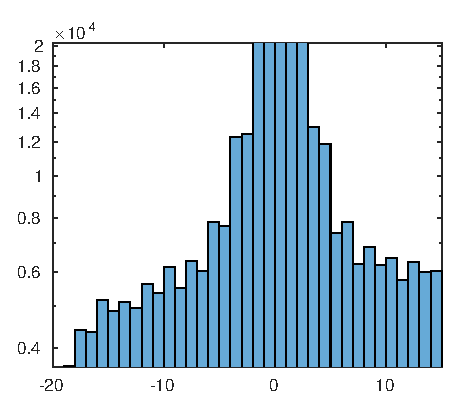
\includegraphics[width=5.5cm]{img/f3-hist.eps}
\caption{Part of a histogram of motion vectors with F3 embedding. Note the unusually higher peaks corresponding to even numbers.}
\label{fig:f3-hist}
\end{wrapfigure}

This embedding strategy leads to an interesting effect called \emph{shrinkage}. Whenever we try to embed a zero bit into $mv_C = -1$ or $mv_C = 1$, the value of $mv_C$ will become 0, so the zero bit will have to be re-embedded again, meaning that F3 will embed more zeroes than ones. 

This is the main weakness of the algorithm. A typical encrypted payload has the same number of zeroes and ones, but since F3 embeds more zeros, values with LSB 0 will be more common (Figure \ref{fig:f3-hist}). 

\subsection{F4}
\label{f4}

F4~\cite{f5} eliminates the weakness of F3 by using a different strategy for embedding into negative values of $mv_C$. Like F3, $mv_C$ is changed (if required) by decrementing its absolute value. When $mv_C$ is positive, the algorithm ensures its LSB matches that of the payload (just like F3), but when $mv_C$ is negative, the algorithm ensures its LSB \emph{does not} match that of the payload. This mapping is visualised in Figure \ref{fig:f4-mapping} and the pseudocode is listed in Algorithm \ref{alg:f4-embed}.

\begin{algorithm}
\caption{Embedding procedure for \emph{F4}.}
\label{alg:f4-embed}
\begin{algorithmic}
\Procedure {F4-Embed}{$mv_C$, $payload_i$}
\If {$mv_C > 0$ \textbf{and} $\textit{LSB}(mv_C) \neq payload_i$}
    \State $mv_C \gets mv_C - 1$ \Comment {Decrease the absolute value of $mv_C$}
\EndIf
\If {$mv_C < 0$ \textbf{and} $\textit{LSB}(mv_C) = payload_i$}
	\State $mv_C \gets mv_C + 1$ \Comment {Decrease the absolute value of $mv_C$}
\EndIf

\State \Return $mv_C \neq 0$
\EndProcedure
\end{algorithmic}
\end{algorithm}

\begin{figure}[tbh]
\centering
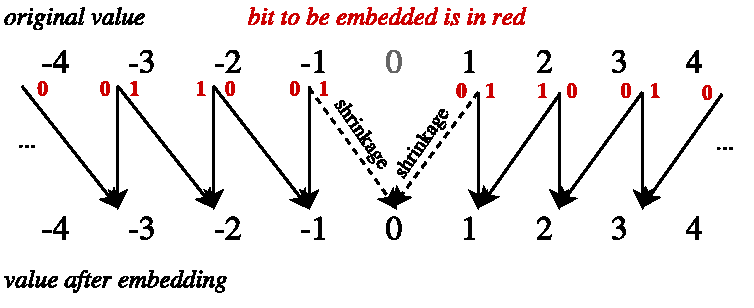
\includegraphics[width=0.7\textwidth]{img/movest_f4_mapping.pdf}
\caption{F4's value mapping depending on the payload bit.}
\label{fig:f4-mapping}
\end{figure}

As we see from Figure \ref{fig:f4-mapping}, shrinkage is no longer exclusively triggered by embedding a zero. Now it can occur when a zero is embedded into value 1 or when a one is embedded into value -1. Assuming both cases occur the same number of times, F4 is not biased towards embedding more zeroes or ones, so is not vulnerable to the same attack. Detectability of this method using the reversion technique is discussed in section \ref{rev-tech}.

\subsection{Randomised Hide \& Seek}
\label{rand-hidenseek}

All of the previous algorithms share a common property: they embed the payload densely in the beginning of a video file, leaving the rest unmodified. We can achieve better undetectability if we spread a small payload across the entire file, making changes less noticeable. 

\emph{Randomised Hide \& Seek}~\cite{bateman} is a modification of the Hide \& Seek algorithm which uses a PRNG to scatter payload bits uniformly across all motion vector components in the video. A simple way to implement this is by randomly choosing an MV component for every payload bit, navigating to the chosen frame and embedding data into the chosen component. Unfortunately, the stream-oriented nature of FFmpeg makes it impossible to switch between frames in this way. To work around this problem, I chose to build a map which assigns every payload bit to a particular (unique) motion vector component ahead of time. This requires knowing the maximum capacity (the number of suitable motion vectors), which is obtained by performing a ``dry run'' beforehand. 

Committing to use a particular motion vector creates a new problem. As explained in \ref{mv-import}, FFmpeg can omit some macroblocks by marking them as ``skipped''. Changing motion vectors in one P-frame can affect which macroblocks are skipped in the following frame. This issue arises when the macroblock pointed to by the mapping becomes unavailable for embedding because it gets omitted. I considered three options to mitigate this issue:
\begin{itemize}
\item Further analyse FFmpeg to be able to reliably predict when ``skipping'' happens  (difficult).
\item Dynamically rebuild the map as data gets embedded. This is a reasonable solution, but will make the algorithm significantly more complex.
\item Use an error correcting code to reconstruct the missing bits. This saves considerable effort, and adds some robustness against tampering, but also increases the payload size due to inclusion of the correction bits.
\end{itemize}

I went with the third option. I chose the widely-used Reed-Solomon~\cite{clarke2002reed} error correcting code, implemented by the \texttt{rscode}\footnote{\url{http://rscode.sourceforge.net/}} library, which operates at a byte-level granularity. Measurements showed that bit errors occur every 400--700 bytes. My default configuration generously specifies 16 error correction (parity) bytes per 239 bytes of data\footnote{The library limits the size of a data block plus a number of parity bytes to 255.}, but it can be adjusted if required. This arrangement is extremely unlikely to fail,\footnote{Assuming that the rate at which errors occur has a normal distribution with mean 550 and variance 150 (in line with the estimate above of 1 error every 400--700 bytes), the probability of a failure is $6.5 \cdot 10^{-6}$. The user can verify that the data can be extracted correctly before transmitting the video.} as it allows correcting up to any 8 incorrect bytes per 239 bytes of payload data.

Extracting the data using this algorithm requires the receiving party's PRNG to output the same sequence of values as the sender's. This is achieved by seeding both sender's and receiver's PRNGs to the same 128-bit value, derived from the user-specified encryption password (in the same way as the encryption key, see \ref{encryption}). Due to the way key derivation functions work, it is impossible to recover the password or the encryption key given only the seed. The receiving party also has to know a bound for the embedding capacity of a video and the embedded file size, but these can be pre-agreed.

For small payload sizes, the algorithm does not produce equal even-odd pairs in the histogram, making many previous attacks ineffective. Although the presence of error correction bits adds a detectable structure to the payload, the embedding algorithm randomly distributes payload bits through the video, hiding it again.

\subsection{Outguess 0.1}
\label{outguess1}

\emph{Outguess 0.1}~\cite{bateman} is essentially the same algorithm as Randomised Hide \& Seek, but it addresses the issue of embedding into ``still'' regions by choosing not to embed into components with value 0 or 1. This is done to avoid the visual analysis attack considered in section \ref{msteg}. Its footprint is evaluated in section \ref{eval-var-emb-cap}.

\subsection{Xu's algorithm}
\label{xu-alg}

The project also implements an algorithm that was designed specifically for motion vectors. Xu \emph{et al.} \cite{xu2006steganography} argue that data should be embedded:
\begin{itemize}
\item Only into motion vectors whose length exceeds a certain threshold, as it would introduce less distortion.
\item Into either $x$ or $y$ component depending on the phase of the motion vector $\theta = \tan^{-1}(y/x)$:
    \begin{itemize}
    \item If $\theta$ is acute, the horizontal component is modified ($x$).
    \item If $\theta$ is obtuse, the vertical component is modified ($y$).
    \end{itemize}
\item By incrementing the chosen component so that it's LSB matches that of the payload bit.
\item 4 times per GOP\footnote{GOP (Group of Pictures) is a series of inter-frames between successive I-frames.} to ``resist video processing''; the starting and ending position of each segment should be recorded in an I-frame using classic image steganography methods.
\end{itemize}

Some of the design decisions made by Xu's algorithm\footnote{The project proposal and progress report refer to this as Zhang's algorithm (2001)~\cite{zhang2001video}. Xu's algorithm (2006)~\cite{xu2006steganography} is a new iteration of the same technique.} are questionable, so I implemented my own take on this technique (\texttt{MVSteg}), with the following differences:
\begin{itemize}
\item $\theta = 90^{\circ}$ is not a good decision boundary: if a motion vector has a large positive $y$ component, but a small positive $x$ component, modifying the larger one would result in a smaller relative change. However, Xu's algorithm would still choose $x$ component, because $\theta$ is an acute angle in this case.

Therefore I chose to embed data into the largest of the two components. If the $x$ and $y$ components are equal, the bit is embedded into both. 

\item Incrementing the chosen component can cause issues if the new value points beyond the edge of the frame. Therefore I chose to decrement the absolute value of the component instead, like F4.

\item Embedding data four times can expose a pattern that may be detected by a steganalyst. I chose not to implement this approach and embed the data sequentially instead.
\end{itemize}

The two algorithms---the original and my modification---are compared in the Evaluation chapter, section \ref{breaking-xu}.

\section{Testing}

In addition to manual testing, unit tests were written to test the implementation. I used the popular Google Test framework~\cite{googletest} to implement small and maintainable tests for my C/C++ code. Components of the system are tested independently via their public interfaces.

Tests cover:
\begin{itemize}
\item Encrypted file access --- ensures that data is correctly encrypted and decrypted during reads and writes, when enabled. Tests use the NIST-recommended AES-CTR test vectors~\cite[Appendix F, Sect. 5.5]{dworkin2001nist}.
\item Embedding algorithms --- ensure algorithms correctly modify and extract data from motion vectors, including typical edge cases for each algorithm.
\item C API (automated integration test) --- ensure the whole steganography library can be successfully used though the API. Tests initialise the library, simulate FFmpeg calls and verify the results.
\end{itemize}

\bigskip
\subsubsection*{Summary}
This chapter described the design and the implementation details of the steganography and steganalysis software. The next chapter will review the project's achievements, cover remaining aspects of detectability evaluation, and evaluate the embedding capacity and speed properties of the system.

% Evaluation
\cleardoublepage
\chapter{Evaluation}

\textit{This chapter evaluates the software against the initial requirements and presents more steganalytic results. The detectability properties using Xu's algorithm, accuracy of the reversion technique classifier, and effectiveness of varying the embedding capacity are discussed. I also discuss secondary properties of steganographic systems, such as the embedding capacity and speed.
}

\section{Satisfaction of requirements}

Overall, the project was a success. All requirements described in sections \ref{req-steg-app} and \ref{req-steg-suite} were met. This section presents a quick review of the software, having these requirements in mind.

\subsection{Steganographic application}

The developed steganography software is able to reliably modify and extract motion vector data from MPEG video files. I obviated the need to implement my own video codec by integrating with FFmpeg (see section \ref{integrate-ffmpeg}). As well as being an impractically large amount of work, writing my own codec may have ramifications for security. My implementation may leave detectable traces in a video file which would reveal the use of steganography. The software consists of 3 deliverables: encoder and decoder applications for the user to perform embedding, and a steganography library that can be used separately though an API. The library implements 8 LSB embedding algorithms (see section \ref{emb-alg}). The payload can be encrypted with 256-bit AES--CTR encryption using a user-supplied password. 

\subsection{Steganalysis suite}

The steganalysis suite provides, in Matlab, facilities for extracting and processing motion vector data, as well as a variety of general attacks for detecting embedded payloads. The following functionality is available:

\begin{multicols}{2}
\begin{itemize}
\item \texttt{loadmvs}, \texttt{typedmvs} --- extraction and filtering of motion vector data;
\item \texttt{lsbplane}, \texttt{plot2d} --- extraction and visualisation of the LSB plane;
\item \texttt{aggregateIntoBytes}, \texttt{seqbytes} --- groups extracted bits into bytes;
\item \texttt{mvhist} --- pre-adjusted histogram to view motion vector data (like in Figure \ref{fig:histogram-example});
\item \texttt{chiSquareAttack} --- compute the embedding probability in the first 1--100\% of the data;\\
\item \texttt{patternSearch} --- find the most likely locations of the pattern in the data;
\item \texttt{known-attacks/} --- examples attacks on implemented algorithms;
\item \texttt{*svmtraining} --- reversion technique SVM training scripts;
\item \texttt{computeSadFreqs} --- SAD frequency computation for the reversion attack.
\end{itemize}
\end{multicols}

Implementation details are discussed in section \ref{steg-tech}, and the effectiveness of the attacks is demonstrated in sections \ref{emb-alg} and \ref{rem-detect-eval}. In-line method documentation is provided on how to use the implemented routines and interpret the results. 

\section{Detectability of embedding}
\label{rem-detect-eval}

Perhaps the most important aspect to consider when evaluating a steganographic system is whether the embedding is detectable. Some of the detectability evaluation was done in the previous chapter to justify further algorithm design improvements, which also allowed evaluating how effective the implemented steganalysis techniques are. This section covers remaining steganalysis.

\subsection{Detecting Xu's algorithm's embedding}
\label{breaking-xu}

I discovered a number of apparent flaws in Xu's algorithm (see section \ref{xu-alg}), so I implemented an improved version of the algorithm, which I called \texttt{MVSteg}.

One of my own improvements is the component selection policy: claiming it disturbs the motion less, the original Xu's algorithm embeds the payload bit into the $x$ component if the phase of the motion vector is acute, otherwise it uses the $y$ component. However, in the presence of a motion vector with a large $y$ component and a small $x$ component (yielding an acute phase), a small marginal change in $x$ results in a large relative disturbance to the motion. MVSteg always modifies the largest component of the motion vector, making the relative change less significant.

Figure \ref{fig:xualg-mvsteg-visual} shows an example of some visual artefacts\footnote{Movest does not modify the prediction error, which makes detecting such artefacts easier. However, if it did, it would still be possible to spot this, because the prediction error would have been unusually large.} produced by Xu's algorithm which are not present when using MVSteg.

\begin{figure}[tbh]
\centerline{
\begin{subfigure}[t]{4cm}
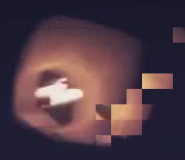
\includegraphics[width=4cm]{img/xualg-visual.png}
\end{subfigure}
~
\begin{subfigure}[t]{4cm}
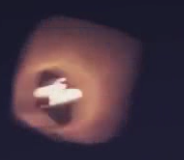
\includegraphics[width=4cm]{img/mvsteg-visual.png}
\end{subfigure}
}
\caption{A frame, showing a sky lantern, containing embedding by Xu's algorithm (left) and MVSteg (right).}
\label{fig:xualg-mvsteg-visual}
\end{figure}

Xu \emph{et al.} also suggest embedding the same chunk of payload data four times at different locations to provide resilience against data corruption. To guide decoding, these locations are stored an I-frame using classical image steganography methods. Unfortunately, this creates a recurring pattern in the LSBs of the used motion vectors, providing an opportunity for attack. I simulated such embedding in the presence some bit corruptions in an attempt to find such repetition. Figure \ref{fig:4xembed} shows a successful result of finding a repeating pattern at four locations, with peaks corresponding to the positions where the pattern closely matches the recovered string\footnote{The sum of squared differences between a pattern and the recovered string is close to zero.}. MVSteg embeds data only once, and hence does not contain exploitable data repetition patterns.

\begin{figure}[tbh]
\centering
\begin{minipage}[t]{.45\textwidth}
  \centering
  \captionsetup{width=\textwidth}
  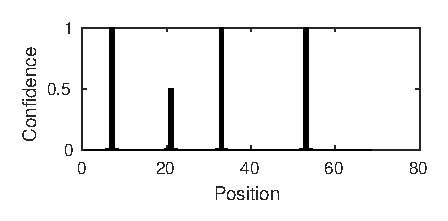
\includegraphics[scale=0.9]{img/4xembed.eps}
  \caption{Positions of repeated embedding. Lower bar corresponds to an inexact match.}
  \label{fig:4xembed}
\end{minipage}%
\quad
\begin{minipage}[t]{.45\textwidth}
  \vspace{-5.14em}
  \captionsetup{width=\textwidth}
  \begingroup
    \fontsize{11pt}{12pt}\selectfont
    \centering
    \begin{alltt}
 {\color{blue}[mpeg4 @ 0x7fc9dc247380]}
            {\color{red}ac-tex damaged at 53 0}
 {\color{blue}[mpeg4 @ 0x7fc9dc247380]}
                   {\color{red}Error at MB: 53}

    \end{alltt}
  \endgroup
  \caption{Macroblock corruption reported by the \texttt{vlc} media player.}
  \label{fig:vlc-corruption}
\end{minipage}
\end{figure}

Xu's algorithm embeds payload bits in motion vectors by incrementing the selected component. For motion vectors near the edge of the frame, such increments can cause the vector to point outside the frame and produce decoding errors which expose the tampering. Figure \ref{fig:vlc-corruption} shows the error that the codec reports when playing such a damaged video. MVSteg's use of F4's decrementing motion vector scheme avoids this problem, also making it resistant to $\chi^2$ and histogram attacks (see sections \ref{steg-tech}, \ref{f4}). Given all these findings, I would advise against using Xu's algorithm in practice.

\subsection{Reversion technique}
\label{rev-tech}

The reversion technique (see section \ref{rev-tech-theory}) considers differences between respective motion vectors of the original and the re-encoded (transcoded) video. Evaluating the effectiveness of this technique requires training a linear SVM classifier. For this application, SVM does not require large datasets to give good results~\cite{cao2012video}, so I have obtained a dataset of 56 freely-available stock videos. The videos were selected to exhibit various degrees of motion, such as slow cloud movements or chaotic city timelapses. Half of those were chosen to become stego videos, so that the ratio between stego and non-stego videos is 50:50 (balanced dataset).

For each embedding algorithm, the training and evaluation is done as follows:
\begin{itemize}
\item To generate the initial dataset of videos, Movest's encoder is used to embed random data into the 28 stego-videos at their full capacity. The remaining 28 non-stego videos are also passed though the encoder without embedding data.
\item To obtain transcoded videos, all previously created videos are passed through the encoder again, letting FFmpeg recompute motion vectors.
\item Motion vectors are extracted from both sets of videos.
\item Motion vector data is imported into Matlab and frequencies of SAD values are computed using the steganalysis suite's \texttt{computeSadFreqs.m} function.
\item Frequency data, together with a labelling whether it came from a stego or a non-stego video, is passed into Matlab's \texttt{fitcsvm} function to train an SVM.
\item Since the dataset is relatively small, the system performs 100 runs of \emph{k-fold cross validation}~\cite{ai2-notes}, with $k = 8$, to estimate the classification accuracy. This is a common technique for evaluating classifiers, provided by Matlab's \texttt{crossval} function.

\end{itemize}

\subsubsection*{8-fold cross validation} 

The data set is randomly partitioned into 8 bins of 7 videos each. For each bin, the other 7 are used to train the classifier, which is then applied to the videos in the target bin and the accuracy is computed.\footnote{Using $k = 8$ (close to recommended $k = 10$) allows having a sufficiently large test set for every iteration.} The average accuracy over all iterations is the result.

Since the resulting accuracy measure is susceptible to unusually favourable random partitioning, the process is repeated 100 times to obtain a 95\% confidence interval for the mean accuracy.

Table \ref{tbl:rev-tech} presents the obtained classification accuracy for each embedding algorithm.

\begin{table}[tbh]
\bgroup
\def\arraystretch{1.3}
\centerline{
\begin{tabular}{|l|c|}
\hline
\textbf{Embedding algorithm} & \textbf{Classification accuracy, 95\% CI} \\
\hline
\textit{Random guess (baseline)} & $50\%$ \\
Hide \& Seek & $100.00\% \pm 0.00\%$ \\ 
MSteg & $92.84\% \pm 0.04\%$ \\ 
F3 & $93.45\% \pm 0.32\%$ \\ 
F4 & $93.25\% \pm 0.16\%$ \\
Xu's algorithm & $63.93\% \pm 0.54\%$ \\
MVSteg & $62.96\% \pm 0.57\%$ \\
\hline
\end{tabular}
}
\egroup
\caption{Reversion technique classifier performance against each sequential embedding algorithm implemented.}
\label{tbl:rev-tech}
\end{table}

The results are surprisingly good, which means this technique is suitable for automated steganalysis. It appears that the accuracy result for each algorithm is similar to the proportion of motion vectors it modifies. The classifier shows over 90\% accuracy for the first four algorithms, suggesting they are easily detectable when the full embedding capacity is used. To mitigate this, one can either use MVSteg, or embed less data, as discussed in the following section.

\subsection{Varying embedding capacity}
\label{eval-var-emb-cap}

Many of the previous attacks, such as the $\chi^2$ attack, exploit a cumulative effect produced when payload bits are embedded close together. Such attacks can be thwarted by spreading the payload uniformly across the cover video.

To evaluate this approach, I tested the $\chi^2$ attack and the reversion technique classifier for MSteg (see \ref{msteg}) against Outguess 1.0\footnote{As discussed in \ref{outguess1}, Outguess 1.0 is the randomised version of MSteg.} at different capacity usage levels. A fresh dataset (not used for classifier training) containing 10 videos was used. Table \ref{tbl:detect-outguess} shows how many stego-videos were detected by each steganalysis. 

\begin{table}[tbh]
\bgroup
\def\arraystretch{1.3}
\centerline{
\begin{tabular}{|l|c|c|}
\hline
\textbf{Embedding capacity} & \textbf{RT Classifier} & $\chi^2$ \textbf{attack} \\
\hline
\textit{0\%} & 0/10 & 0/10   \\
10\% & 1/10 & 0/10   \\
20\% & 1/10 & 0/10   \\
30\% & 1/10 & 0/10   \\
40\% & 1/10 & 0/10   \\
50\% & 4/10 & 0/10   \\
60\% & 6/10 & 0/10   \\
70\% & 7/10 & 0/10   \\
80\% & 7/10 & 0/10   \\
90\% & 8/10 & 2/10   \\
\textit{100\%} & 9/10 & 10/10 \\
\hline
\end{tabular}
}
\egroup
\caption{Detectability of Outguess 0.1 embedding at various embedding capacities.}
\label{tbl:detect-outguess}
\end{table}

The table also includes an entry for 0\% setting (no data embedded) to verify that the attacks do not produce false positives. These data suggest that the reversion technique classifier starts being effective at 50--60\% embedding capacity and the $\chi^2$ attack is only effective from 90\%. The embedding is therefore undetectable using implemented steganalysis techniques, provided less than half of the video's embedding capacity is used.

\section{Detectability by humans (study)}
\label{exp-human-subj}

\subsection{Study hypothesis}

A study was conducted to test whether human participants are able to distinguish between a stego and a non-stego video when the prediction error is not modified. To test this, I measured how often participants could correctly select the stego video given three ostensibly identical videos. I hypothesise that humans are not able to tell the videos apart (null hypothesis).

\subsection{Experimental procedure}

In each of 10 trials, the participant was given three ostensibly identical videos under 30 seconds in length, one of which containing a hidden payload. They had to choose which video they thought was modified and write its letter into the experiment answer sheet. Using three videos, as opposed to two, eliminates the problematic situation in which the participant sees that the videos are different, but is unable to tell which one actually contains embedding.\footnote{The original experiment description in the project proposal overlooked this issue and stated that 2 videos will be used. I would like to thank the Computer Laboratory Ethics Committee for advising me on this matter.}

To increase chances of successful detection and more closely simulate a real-life steganalysis setting, the following measures were taken:
\begin{itemize}
\item Test subjects were computer-literate. Most were computer science undergraduates.
\item Embedding was done using the Hide \& Seek algorithm, which leaves a significant footprint by modifying every motion vector (see steganalysis in section \ref{hide-n-seek}). The full embedding capacity of every video was used to embed random data to simulate an encrypted payload. 
\item Participants had full control over the playback, meaning they could watch videos however they liked: sequentially, side-by-side, repeatedly replay certain parts, inspect file sizes, zoom into certain regions of a video, use either their own or my screen \emph{etc.}
\item The first trial contained an artificially corrupted video (motion vectors were changed more drastically) to give participants an idea of what kind of visual footprint to expect. 
\end{itemize}

Videos were emotionally neutral, and free from flashing, distressful, disturbing, offensive or otherwise unsettling images. No personal data about the participants was collected.

\subsection{Results}

The data obtained from the experiment is presented in Table \ref{tbl:detect-exp-res}. 

\begin{table}[tbh]
\centering
\bgroup
\def\arraystretch{1.3}
\begin{tabular}{|l|c|c|c|c|c|c|c|c|c|c|}
\hline
\textbf{Video \#} & \textbf{1} & \textbf{2} & \textbf{3} & \textbf{4} & \textbf{5} & \textbf{6} & \textbf{7} & \textbf{8} & \textbf{9} & \textbf{10}\\
\hline
\textit{Correct answer} & \textit{B} & \textit{C} & \textit{C} & \textit{A} & \textit{B} & \textit{B} & \textit{A} & \textit{C} & \textit{B} & \textit{A}\\
\hline
Participant \#1  & B & C & C & B & A & C & A & B & A & C \\
Participant \#2  & B & A & B & C & C & B & A & B & A & A \\
Participant \#3  & B & C & B & A & C & A & A & B & A & C \\
Participant \#4  & B & A & A & B & B & C & C & A & B & C \\
Participant \#5  & B & A & C & B & C & A & A & C & B & C \\
Participant \#6  & B & C & C & A & A & B & C & C & C & B \\
Participant \#7  & B & A & A & C & A & C & C & C & C & A \\
Participant \#8  & B & B & A & C & A & A & B & A & C & C \\
Participant \#9  & B & C & B & C & A & C & A & C & C & C \\
Participant \#10 & B & A & A & C & A & C & B & C & A & C \\
Participant \#11 & B & B & B & C & C & B & C & A & C & C \\
Participant \#12 & B & C & A & A & B & B & B & A & B & B \\
\hline
\end{tabular}
\egroup
\caption{Results of the distinguishability of video steganography experiment. Column 1 corresponds to the demo trial with an evidently corrupted video, so it is excluded from the analysis.}
\label{tbl:detect-exp-res}
\end{table}

To be able to interpret the data, I defined a theoretical model to fit the experiment. Let $n$ be the number of answers that participants gave and $X_i$ ($i \in [1, n]$) denote whether an answer was correct, \emph{i.e.} $X_i = 1$ if a participant correctly identified the stego video in a trial and $0$ otherwise. If the null hypothesis holds, the participants' answers will be indistinguishable from random guesses, meaning the $X_i$ can be modelled as a random variable with $\mathbb{P}(X_i = 1) = 1/3$. That is, the $X_i$'s follow Bernoulli distribution with $p = 1/3$. 

To aggregate, I compute the sum of all $X_i$: $Y = \sum^n_{i=1} X_i$. For sufficiently large $n$, $Y$ follows the Binomial distribution with parameters $(n, p)$~\cite[p.~53]{papoulis2002probability}. Then, by the de Moivre--Laplace theorem, $Y$ can be approximated by a normal distribution with mean $np$ and variance $np(1-p)$~\cite[p.~105]{papoulis2002probability}. This allows us to put 95\% confidence bounds on the value of $Y$~\cite[p.~316--318]{ai2-notes}:
\[ np - 1.96 \sqrt{np(1-p)}  \leq Y \leq  np + 1.96 \sqrt{np(1-p)} \]

If $Y$, obtained from the data set, does not lie in this range, the null hypothesis can be rejected with 95\% confidence.

The data contains 108 answers ($n = \text{\# of participants} \times \text{\# of trials}$), so, according to the formula above, I expect $Y$ to be within the range $36 \pm 5$. The data has 32 correct answers, which is within that range, so it \emph{cannot} be concluded that humans \emph{are} able to identify implemented video steganography. This suggests that the visual footprint produced by not modifying prediction error is not detectable by humans.

\section{Embedding capacity and speed}

A steganographic system also has secondary characteristics worthy of evaluation: embedding capacity and speed. Capacity depends on the number of P-frames, macroblocks (defined by the resolution), and suitable motion vectors (see \ref{mv-emb-space}). The proportion of suitable motion vectors can vary significantly depending on the type of motion in a video, and on what algorithm is used. For instance, MVSteg performs worse on videos with little or slow motion because it only embeds into sufficiently long motion vectors (see \ref{xu-alg}).

To estimate the capacities a user might reasonably expect, I measured embedding capacity per second on a dataset of 53 HD ($1280 \times 720$) videos with varying degrees of motion, averaged over a representative span of 15 seconds. Figure \ref{fig:capacities} presents a box plot of measured capacities for each embedding algorithm. Hide \& Seek achieves an impressive 20~KB/s median embedding capacity; MSteg's, F3's and F4's median result is 6--8~KB/s, and Xu's algorithm and MVSteg have the lowest values of 1~KB/s. 

\begin{figure}[tbh]
\centerline{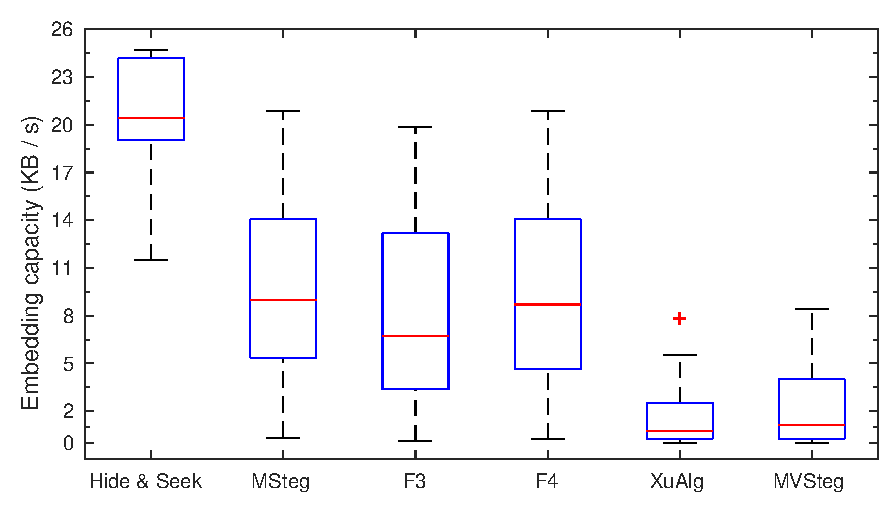
\includegraphics{img/capacities.eps}}
\caption{Box plot showing possible embedding capacities (KB/s) for every algorithm.}
\label{fig:capacities}
\end{figure}

Video encoding is the most computationally expensive part of the Movest encoder, so the time taken by steganography routines is relatively negligible. I did not observe any significant decrease in the encoding speed, even when using payload encryption. The most noticeable slowdown in the encoder is the initialisation overhead of the Randomised Hide \& Seek algorithm to build the payload bit to MV component mapping (see section \ref{rand-hidenseek}).

\bigskip\bigskip
\subsection*{Summary}
This chapter evaluated the implementation with respect to initial requirements and showed that they were met. The detectability, capacity, and speed properties of steganographic systems were investigated. The following chapter summarises the undertaken work and suggests future work.

% Conclusions
\cleardoublepage
\chapter{Conclusions}

\section{Accomplishments}

Overall, the project achieved its aim of implementing and evaluating existing LSB steganography methods using motion vectors. Steganographic systems were evaluated based on embedding capacity, speed, and detectability. Detectability was evaluated using implemented steganalysis methods and by carrying out an experiment on human subjects.

A library for performing steganography and related video processing (such as accessing and modifying motion vectors) applications were developed. The steganalysis suite, implemented using Matlab, provides facilities for extraction and analysis of motion vectors and offers classic and motion vector-specific attacks against embedding algorithms.

With the benefit of hindsight, I would have implemented the FFmpeg integration prior to starting the project and used it as a starting point. This would have allowed focusing entirely on steganography, giving more time to explore useful extensions.

\section{Future directions}

Many promising avenues for further improvement were not explored due to time constraints:
\begin{itemize}
\item \textit{Non-LSB embedding algorithms.} Fang \emph{et al.}~\cite{fang2006data} propose to restrict motion vector search to the one of 4 quadrants, allowing conveyance of 2 bits of data per MV. This requires a deeper integration with a video codec than I have so far implemented.
\item \textit{Transcoding resilience.} Embedding schemes that withstand transcoding would be useful for things like communication over social media. Services such as YouTube, Facebook and Tumblr transcode user-uploaded videos before presenting them to other users, destroying any payload hidden in motion vectors. Embedding algorithms that make use of error correcting codes or redundant encoding may be better able to resist this.
\item \textit{Explore MV-specific steganalysis further.} In addition to the reversion technique, described in \ref{rev-tech}, the project would benefit from more motion vector-specific steganalysis methods. A few potential candidates were mentioned in the Introduction chapter: Deng \emph{el al.}~\cite{deng2012digital} argues that neighbouring MVs often have the same motion vectors, making it easy to spot an abnormal motion vector, and Xu \emph{et al.}~\cite{xu2013video} proposed to build a set of vector algebra constraints between MVs across several frames for this purpose.
\item \textit{Improve user interface.} The current CLI could be replaced by a more novice-friendly GUI, providing helpful guidance for inexperienced users who want to start using covert communication. It could include a privacy advice and an automatic algorithm recommendation based on a set of predefined use-cases, the payload size and the video embedding capacity. An HCI trial could be conducted to evaluate whether the interface helps users achieve required communication secrecy level while being educative and easy to use. 
\end{itemize}

\subsection*{Closing remarks}

It has been a fascinating opportunity to explore niche fields of steganography and steganalysis, investigate and compare their research advances and apply explored methods to video coding. The project has achieved its goals, contributing both theoretically and practically, as a review of LSB steganography adapted to motion vectors and as a collection of practical stego tools.

\cleardoublepage
\bibliographystyle{unsrt}
\addcontentsline{toc}{chapter}{Bibliography}
\bibliography{refs}

\appendix
\cleardoublepage
\addcontentsline{toc}{chapter}{Appendix A:\quad Project proposal}
\chapter*{Appendix A: Project proposal}

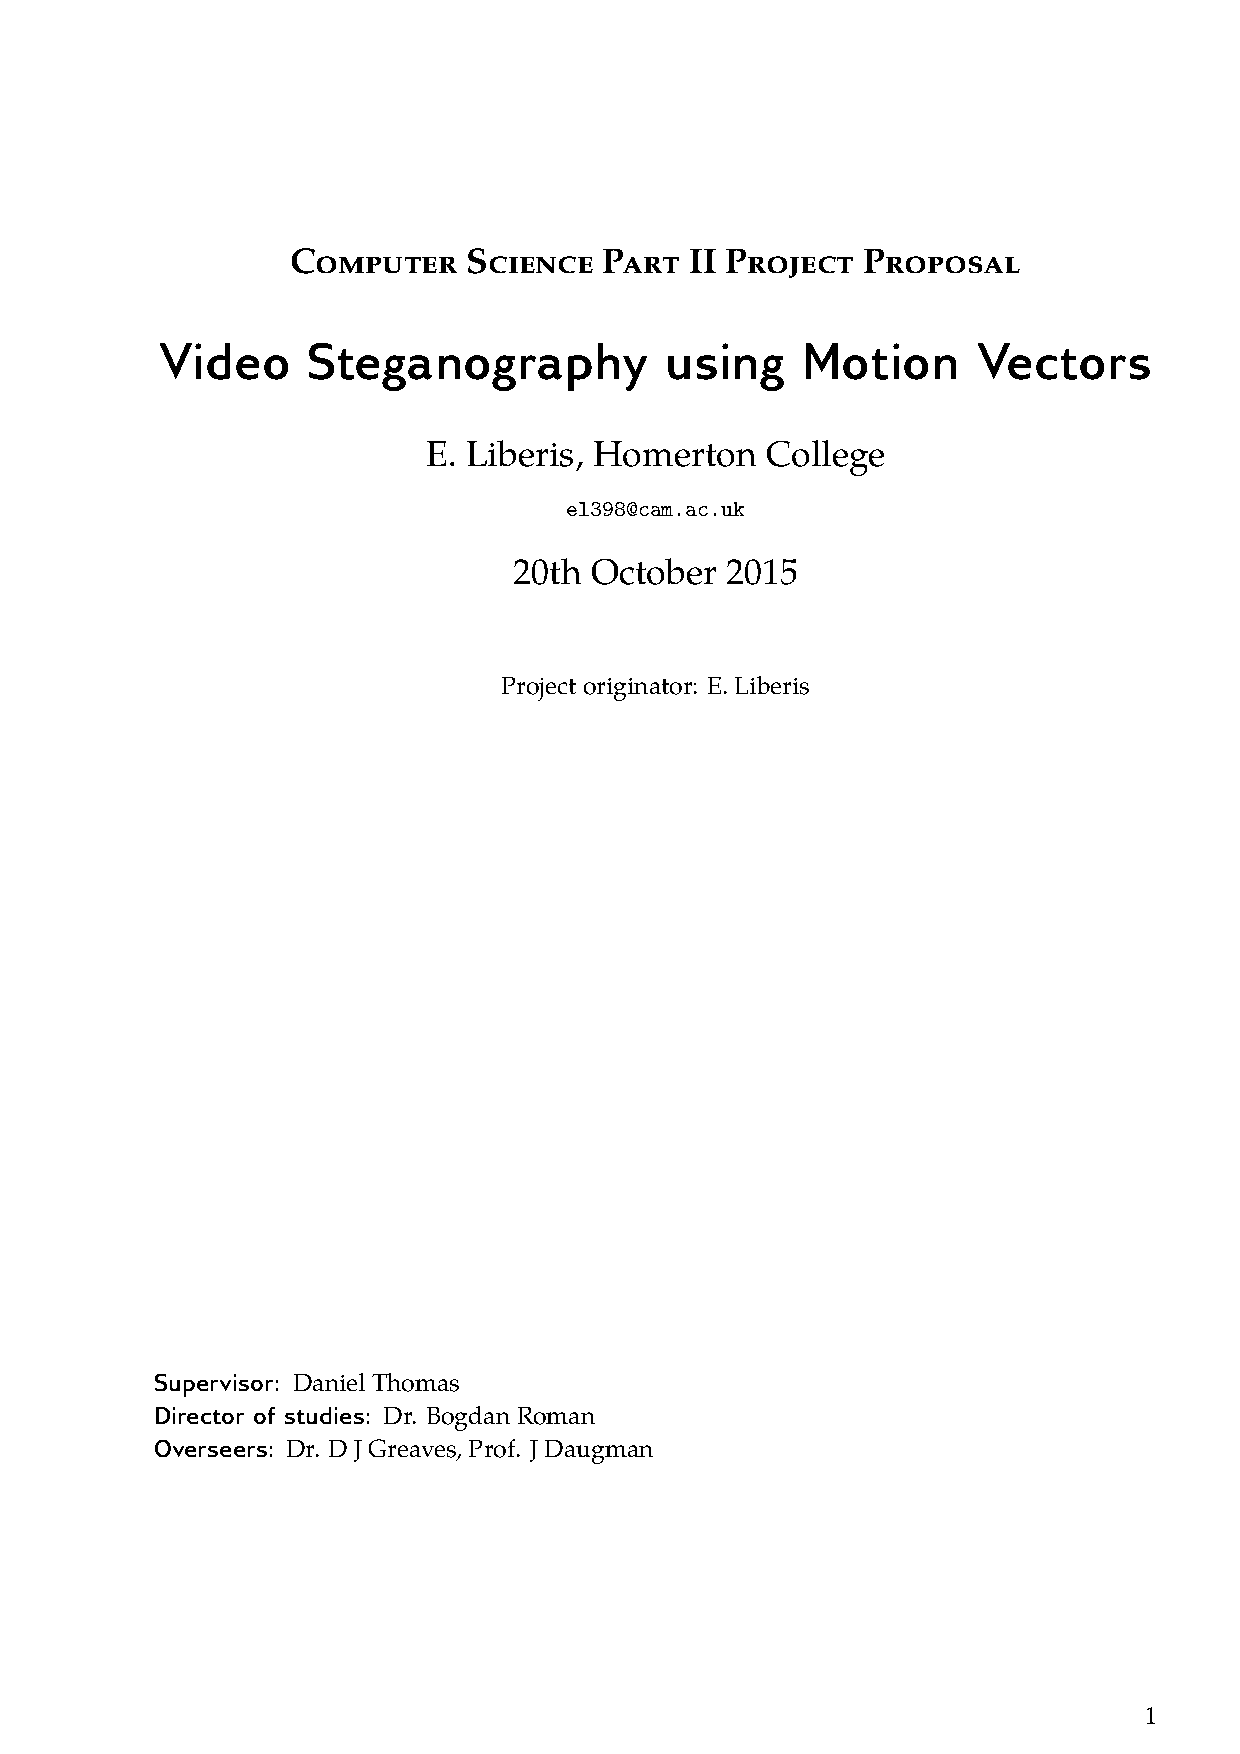
\includepdf[pages={-}]{proposal.pdf}


\end{document}